\documentclass[12pt]{beamer}
\usepackage{amsmath}
\usepackage{mathtools}
\usepackage{multimedia}
\usepackage{hyperref}
\usepackage{booktabs}

\usefonttheme{professionalfonts} % using non standard fonts for beamer
\usefonttheme{serif} % default family is serif
%\documentclass[12pt]{beamerthemeSam.sty}
\usepackage{epsf}
%\usepackage{pstricks}
%\usepackage[orientation=portrait,size=A4]{beamerposter}
\geometry{paperwidth=160mm,paperheight=120mm}
%DT favorite definitions
\def\LL{\left\langle}	% left angle bracket
\def\RR{\right\rangle}	% right angle bracket
\def\LP{\left(}		% left parenthesis
\def\RP{\right)}	% right parenthesis
\def\LB{\left\{}	% left curly bracket
\def\RB{\right\}}	% right curly bracket
\def\PAR#1#2{ {{\partial #1}\over{\partial #2}} }
\def\PARTWO#1#2{ {{\partial^2 #1}\over{\partial #2}^2} }
\def\PARTWOMIX#1#2#3{ {{\partial^2 #1}\over{\partial #2 \partial #3}} }

\def\rightpartial{{\overrightarrow\partial}}
\def\leftpartial{{\overleftarrow\partial}}
\def\diffpartial{\buildrel\leftrightarrow\over\partial}

\def\HC{\column{0.5\textwidth}}
\def\BBC{\begin{columns}}
\def\EEC{\end{columns}}
\def\BCC{\begin{columns}}
\def\ECC{\end{columns}}
\def\BC{\begin{center}}
\def\EC{\end{center}}
\def\BN{\begin{enumerate}}
\def\EN{\end{enumerate}}
\def\BI{\begin{itemize}}
\def\EI{\end{itemize}}
\def\BE{\begin{displaymath}}
\def\EE{\end{displaymath}}
\def\BEA{\begin{eqnarray*}}
\def\EEA{\end{eqnarray*}}
\def\BNEA{\begin{eqnarray}}
\def\ENEA{\end{eqnarray}}
\def\EL{\nonumber\\}

\newcommand{\etal}{{\it et al.}}
\newcommand{\gbeta}{6/g^2}
\newcommand{\la}[1]{\label{#1}}
\newcommand{\ie}{{\em i.e.\ }}
\newcommand{\eg}{{\em e.\,g.\ }}
\newcommand{\cf}{cf.\ }
\newcommand{\BS}{\bigskip}
\newcommand{\etc}{etc.\ }
\newcommand{\atantwo}{{\rm atan2}}
\newcommand{\Tr}{{\rm Tr}}
\newcommand{\dt}{\Delta t}
\newcommand{\op}{{\cal O}}
\newcommand{\msbar}{{\overline{\rm MS}}}
\def\chpt{\raise0.4ex\hbox{$\chi$}PT}
\def\schpt{S\raise0.4ex\hbox{$\chi$}PT}
\def\MeV{{\rm Me\!V}}
\def\GeV{{\rm Ge\!V}}

%AB: my color definitions
%\definecolor{mygarnet}{rgb}{0.445,0.184,0.215}
%\definecolor{mygold}{rgb}{0.848,0.848,0.098}
%\definecolor{myg2g}{rgb}{0.647,0.316,0.157}
\definecolor{A}{rgb}{1.0,0.3,0.3}
\definecolor{B}{rgb}{0.0,1.0,0.0}
\definecolor{C}{rgb}{1.0,1.0,0.0}
\definecolor{D}{rgb}{0.5,0.5,1.0}
\definecolor{E}{rgb}{0.7,0.7,0.7}
\definecolor{abtitlecolor}{rgb}{1.0,1.0,1.0}
\definecolor{absecondarycolor}{rgb}{0.0,0.416,0.804}
\definecolor{abprimarycolor}{rgb}{1.0,0.686,0.0}
\definecolor{Red}           {rgb}{1,0.4,0.4}
\definecolor{Yellow}           {rgb}{1,1,0.0}
\definecolor{Grey}          {cmyk}{.7,.7,.7,0}
\definecolor{Blue}          {cmyk}{1,1,0,0}
\definecolor{Green}         {cmyk}{1,0,1,0}
\definecolor{Brown}         {cmyk}{0,0.81,1,0.60}
\definecolor{Silver}        {rgb}{0.95,0.9,1.0}
\definecolor{Sky}           {rgb}{0.07,0.0,0.2}
\definecolor{Darkbrown}     {rgb}{0.4,0.3,0.2}
\definecolor{Black}         {rgb}{0.0,0.0,0.0}
\definecolor{Orange}         {rgb}{1.0,0.5,0.0}
\definecolor{40Gray}        {rgb}{0.4,0.4,0.5}
\usetheme{Madrid}


\setbeamercolor{normal text}{fg=Silver,bg=Sky}

%AB: redefinition of beamer colors
%\setbeamercolor{palette tertiary}{fg=white,bg=mygarnet}
%\setbeamercolor{palette secondary}{fg=white,bg=myg2g}
%\setbeamercolor{palette primary}{fg=black,bg=mygold}
\setbeamercolor{title}{fg=abtitlecolor}
\setbeamercolor{frametitle}{fg=abtitlecolor}
\setbeamercolor{palette tertiary}{fg=white,bg=Darkbrown}
\setbeamercolor{palette secondary}{fg=white,bg=absecondarycolor}
\setbeamercolor{palette primary}{fg=white,bg=40Gray}
\setbeamercolor{structure}{fg=abtitlecolor}

\setbeamerfont{section in toc}{series=\bfseries}

%AB: remove navigation icons
\beamertemplatenavigationsymbolsempty
\title[Spaceflight since Apollo]{
  \textbf {Spaceflight since Apollo}}

\author [Astronomy 101]{Astronomy 101\\Syracuse University, Fall 2022\\Walter Freeman}

\date{\today}

\begin{document}



\frame{\titlepage}


\frame{\frametitle{\textbf{Announcements: makeups/retakes}}

\large

See email/Blackboard for announcements about lab makeups and quiz retakes.

\BS

Turn your homework (due today) in when you leave class today.

\BS

Please write your name and your TA's name at the top.

}
\frame{\frametitle{\textbf{Announcements: final project submissions}}
	You may submit your final projects:
	\BI
	\item {\bf \color{Red}At the final exam (Tuesday, December 13, 3pm-5pm)}
	\pause
	\item To me in my office, on December 9 (morning)
	\item To me in Holden Observatory, on December 9 (afternoon, 2pm-4pm)
	\item By email to {\tt suast101projects@gmail.com}
	\EI
	
	\BS
	
	\pause
	\BC
	{\color{A}We want to accommodate your creativity. If you have something unusual in mind, let us know and we will work with you.}
	
	\pause\BS\BS
	
	{\color{D}If you are doing something ambitious and realize you need more time, please ask!}
	
	\pause\BS\BS
	
	{\color{B}Please send files as attachments. If you must send links to cloud storage sites, make sure the permissions are set to ``anyone with the link''.}
	
	
	\pause\BS\BS
	
	{\color{C}Remember that creative projects should include a brief artist's statement linking your creative work to the stuff of astronomy or science.}
	
	\EC
}


\frame{\titlepage}

\frame{
	\BC
	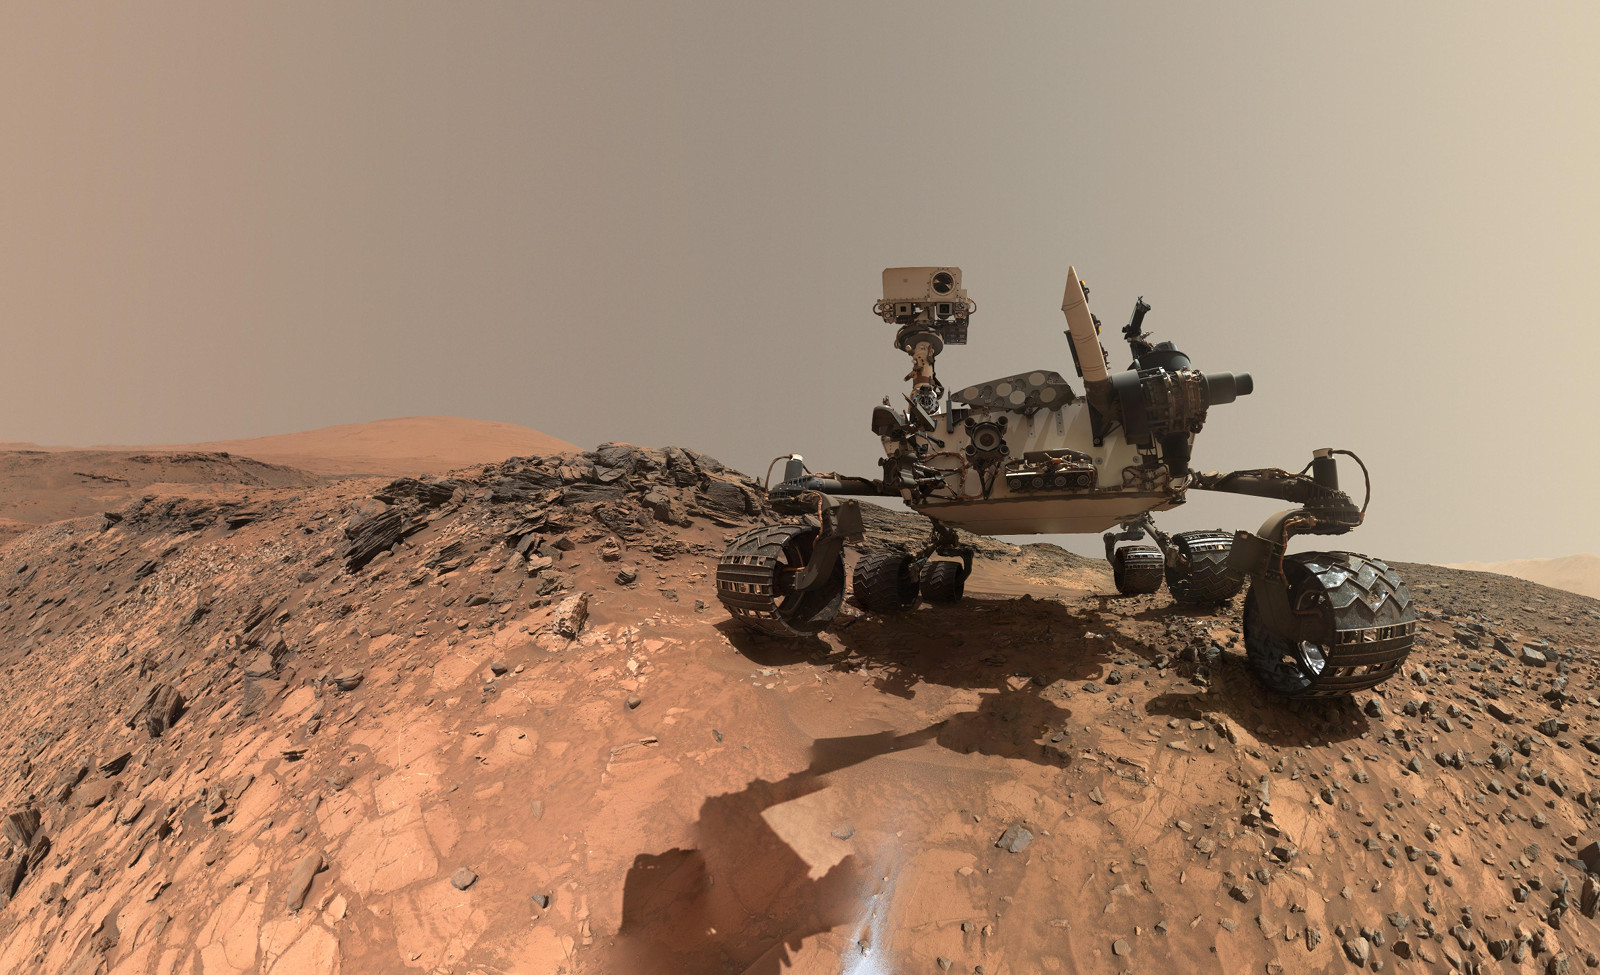
\includegraphics[height=0.8\textheight]{curiosity.jpg}\\
	\it Selfie by the \rm Curiosity \it rover, on the Martian surface
	\EC
}

%\frame{
%	\BC
%	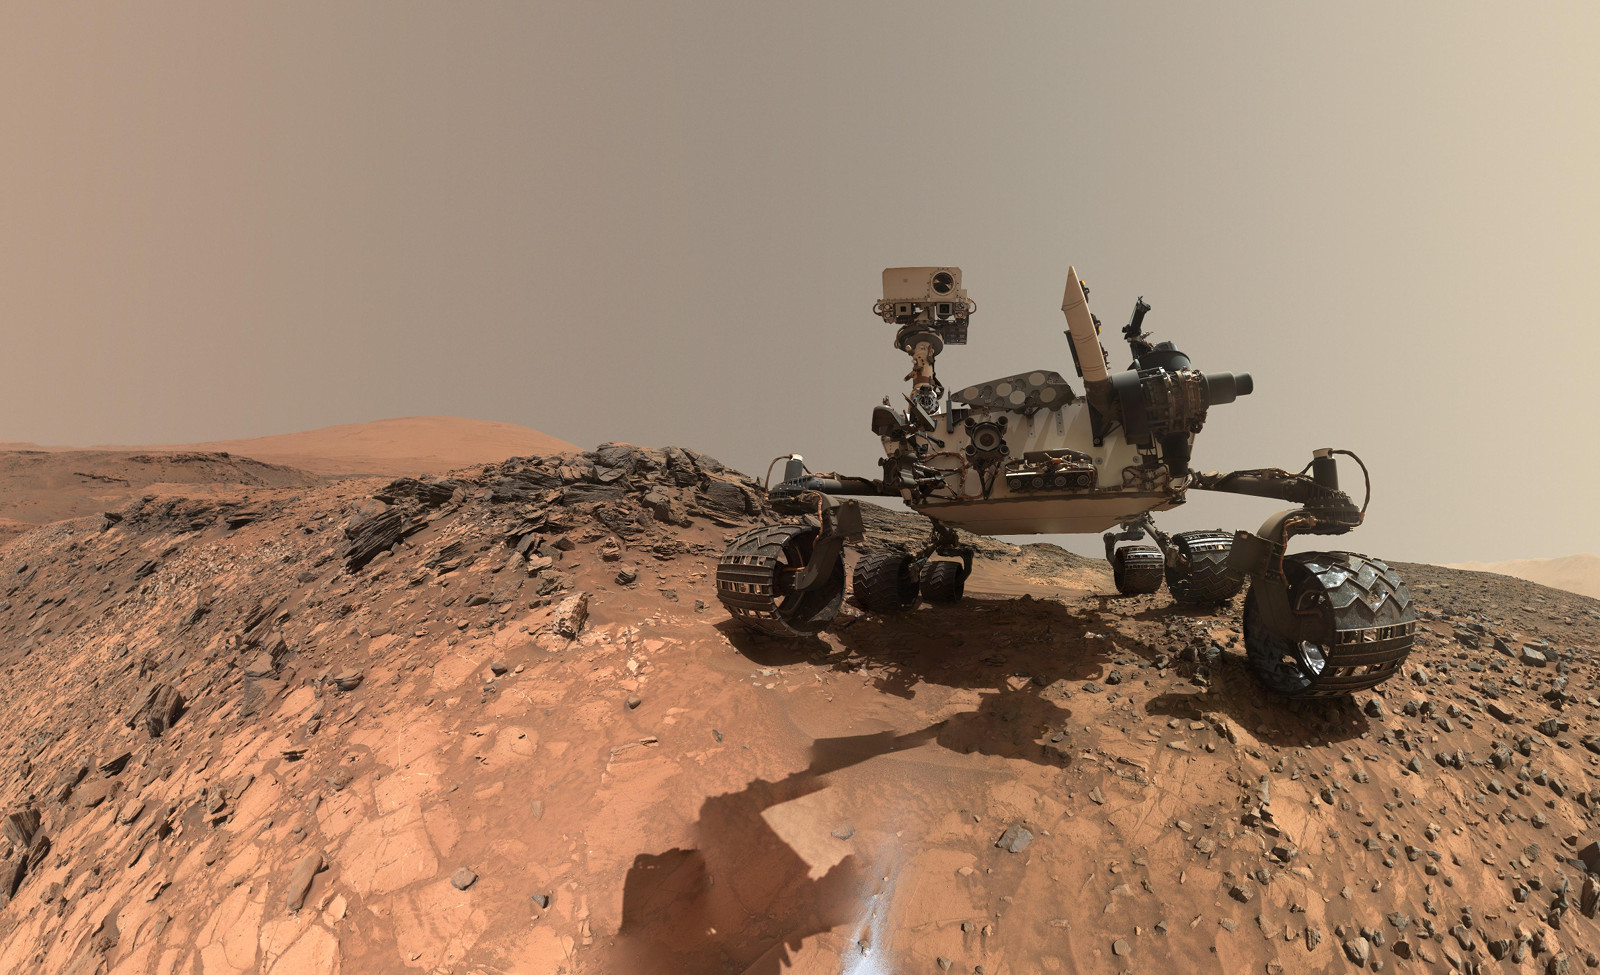
\includegraphics[height=0.8\textheight]{curiosity.jpg}\\
%	\it Selfie by the \rm Curiosity \it rover, on the Martian surface
%	\EC
%}
%




\frame{\frametitle{\textbf{Announcements: final projects}}
	\large
	\BI
	\item I've heard a lot of fantastic ideas for final projects already (and seen a few completed ones)
	\item Remember, your projects are due on the day of the final
	\BI
	\item We'll have a box there for you to submit things
	\item If your project is something best submitted electronically, email it to suast101projects@gmail.com
	\item If your project is something complicated (artwork, etc.), come talk to me; we'll make arrangements
	\item If you take your exams at CDR, get your project to me before/after (I'll be around, and will be in the Physics Clinic after the exam)
	\EI
	\EI
}

\frame{\frametitle{\textbf{Announcements: final project submissions}}
	You may submit your final projects:
	\BI
	\item {\bf \color{Red}At the final exam (Tuesday, December 14, 3pm-5pm)}
	\pause
	\item To the TA's at Holden Observatory on Friday morning, December 10, from 9:30am-2pm
	\item To a box in front of my office, Physics Building 215, on December 10
	\item To your TA's mailbox (for papers and things that will fit)
	\item By email to {\tt suast101projects@gmail.com}
	\EI
	
	\BS
	
	\pause
	\BC
	{\color{A}We want to accommodate your creativity. If you have something unusual in mind, let us know and we will work with you.}
	
	%	\pause\BS\BS
	%	
	%	{\color{B}Please send files as attachments. If you must send links to cloud storage sites, make sure the permissions are set to ``anyone with the link''.}
	%	
	%	
	\pause\BS\BS
	
	{\color{C}Doing something creative and awesome and running out of time? Contact me for an extension; we will grant these for ambitious and creative projects depending on what you're doing and what you need.}
	
	\EC
}

\frame{\frametitle{\textbf{Announcements: take-home lab}}
	\large
	\BC {\color{B} \bf The take-home lab is due this Friday, 9 December.} \EC
	
	\BS\BS
	
	I accidentally wrote ``10 December'' in one place, which is of course a Saturday. So, if you turn it in Monday morning, that's okay too. Put it in your TA's mailbox in the Physics Building.
	
	\BS\BS
	
	If you didn't do it, it is far too late to do it now. It requires actual measurements of the real Sun or Moon; you cannot do it with simulated or borrowed data.
	
	\BS\pause
	
	If you didn't do it, we will make a correction so that missing it doesn't affect your grade too badly.
}


\frame{\frametitle {\textbf{Preparing for the final exam}}
	\large
	\BI
	\item The final exam is next Tuesday, 3PM - 5PM, 13 December
	\item {\color{Red} Section 1 (12:30): Stolkin Auditorium (here) }
	\item {\color{Green} Section 2 (2:00): ({\color{A}not here)}} 
	\item Bring your final projects to the final to submit them
	\EI
	\BS
}

\frame{\frametitle {\bf Preparing for the final exam: review sessions}
	\BI
	\item I'll be holding usual office hours tomorrow and extra help Friday in Holden or the Physics Clinic (12-4 pm).
	\BS
	\item The best things to study and how to use them:
	\BI
	\item \color{A} Previous exercises and homework \pause -- as the tutorials where you gained your skills\pause
	\item \color{B} Previous exams \pause-- as the sorts of ways we evaluated you on these things\pause
	\item \color{C} The study guides \pause-- as a narration of all the course content in one place\pause
	\item \color{D} Your labs \pause-- the high points from them will also be on the final, but {\it there will not be detailed math}
	\EI
	\BS
	\item Next Monday: I'll be in the Physics Clinic as often as I can; so will Clinic TA's
	\BI
	\item \footnotesize I'll send out a note Monday morning/Sunday night with the expected schedule
	\EI
	\item Next Tuesday: will be in and out of the Physics Clinic from 10AM until your exam starts
	\EI
}

%\frame{\frametitle {\bf Grade checking}
%\large
%\BI
%\item I anticipate finishing almost all of my backlog of grading tomorrow morning.
%\item I'll send out an email when this is done; at that point, your grades should be on Blackboard.
%\BI
%\item This doesn't include incidental extra credit.
%\EI
%\BS
%
%\item When I do that, please {\color{Red}check your Blackboard grades for accuracy.} If anything is wrong:
%\BI
%\item If there is a problem with {\it lab grades}, contact your TA 
%\item If there is a problem with {\it paper grades}, contact your TA cc: me
%\item If there is a problem with {\it exam grades}, contact me
%\EI
%\BS
%\item Friday is a good time to tell me about grade issues (bring your papers if you have them) 
%\EI
%}


\frame{\frametitle{\bf 300 BCE: The dream of flight}
	
	\large
	
	
	\BC
	\BS The ancients; flight as hubris...\\\BS
	
	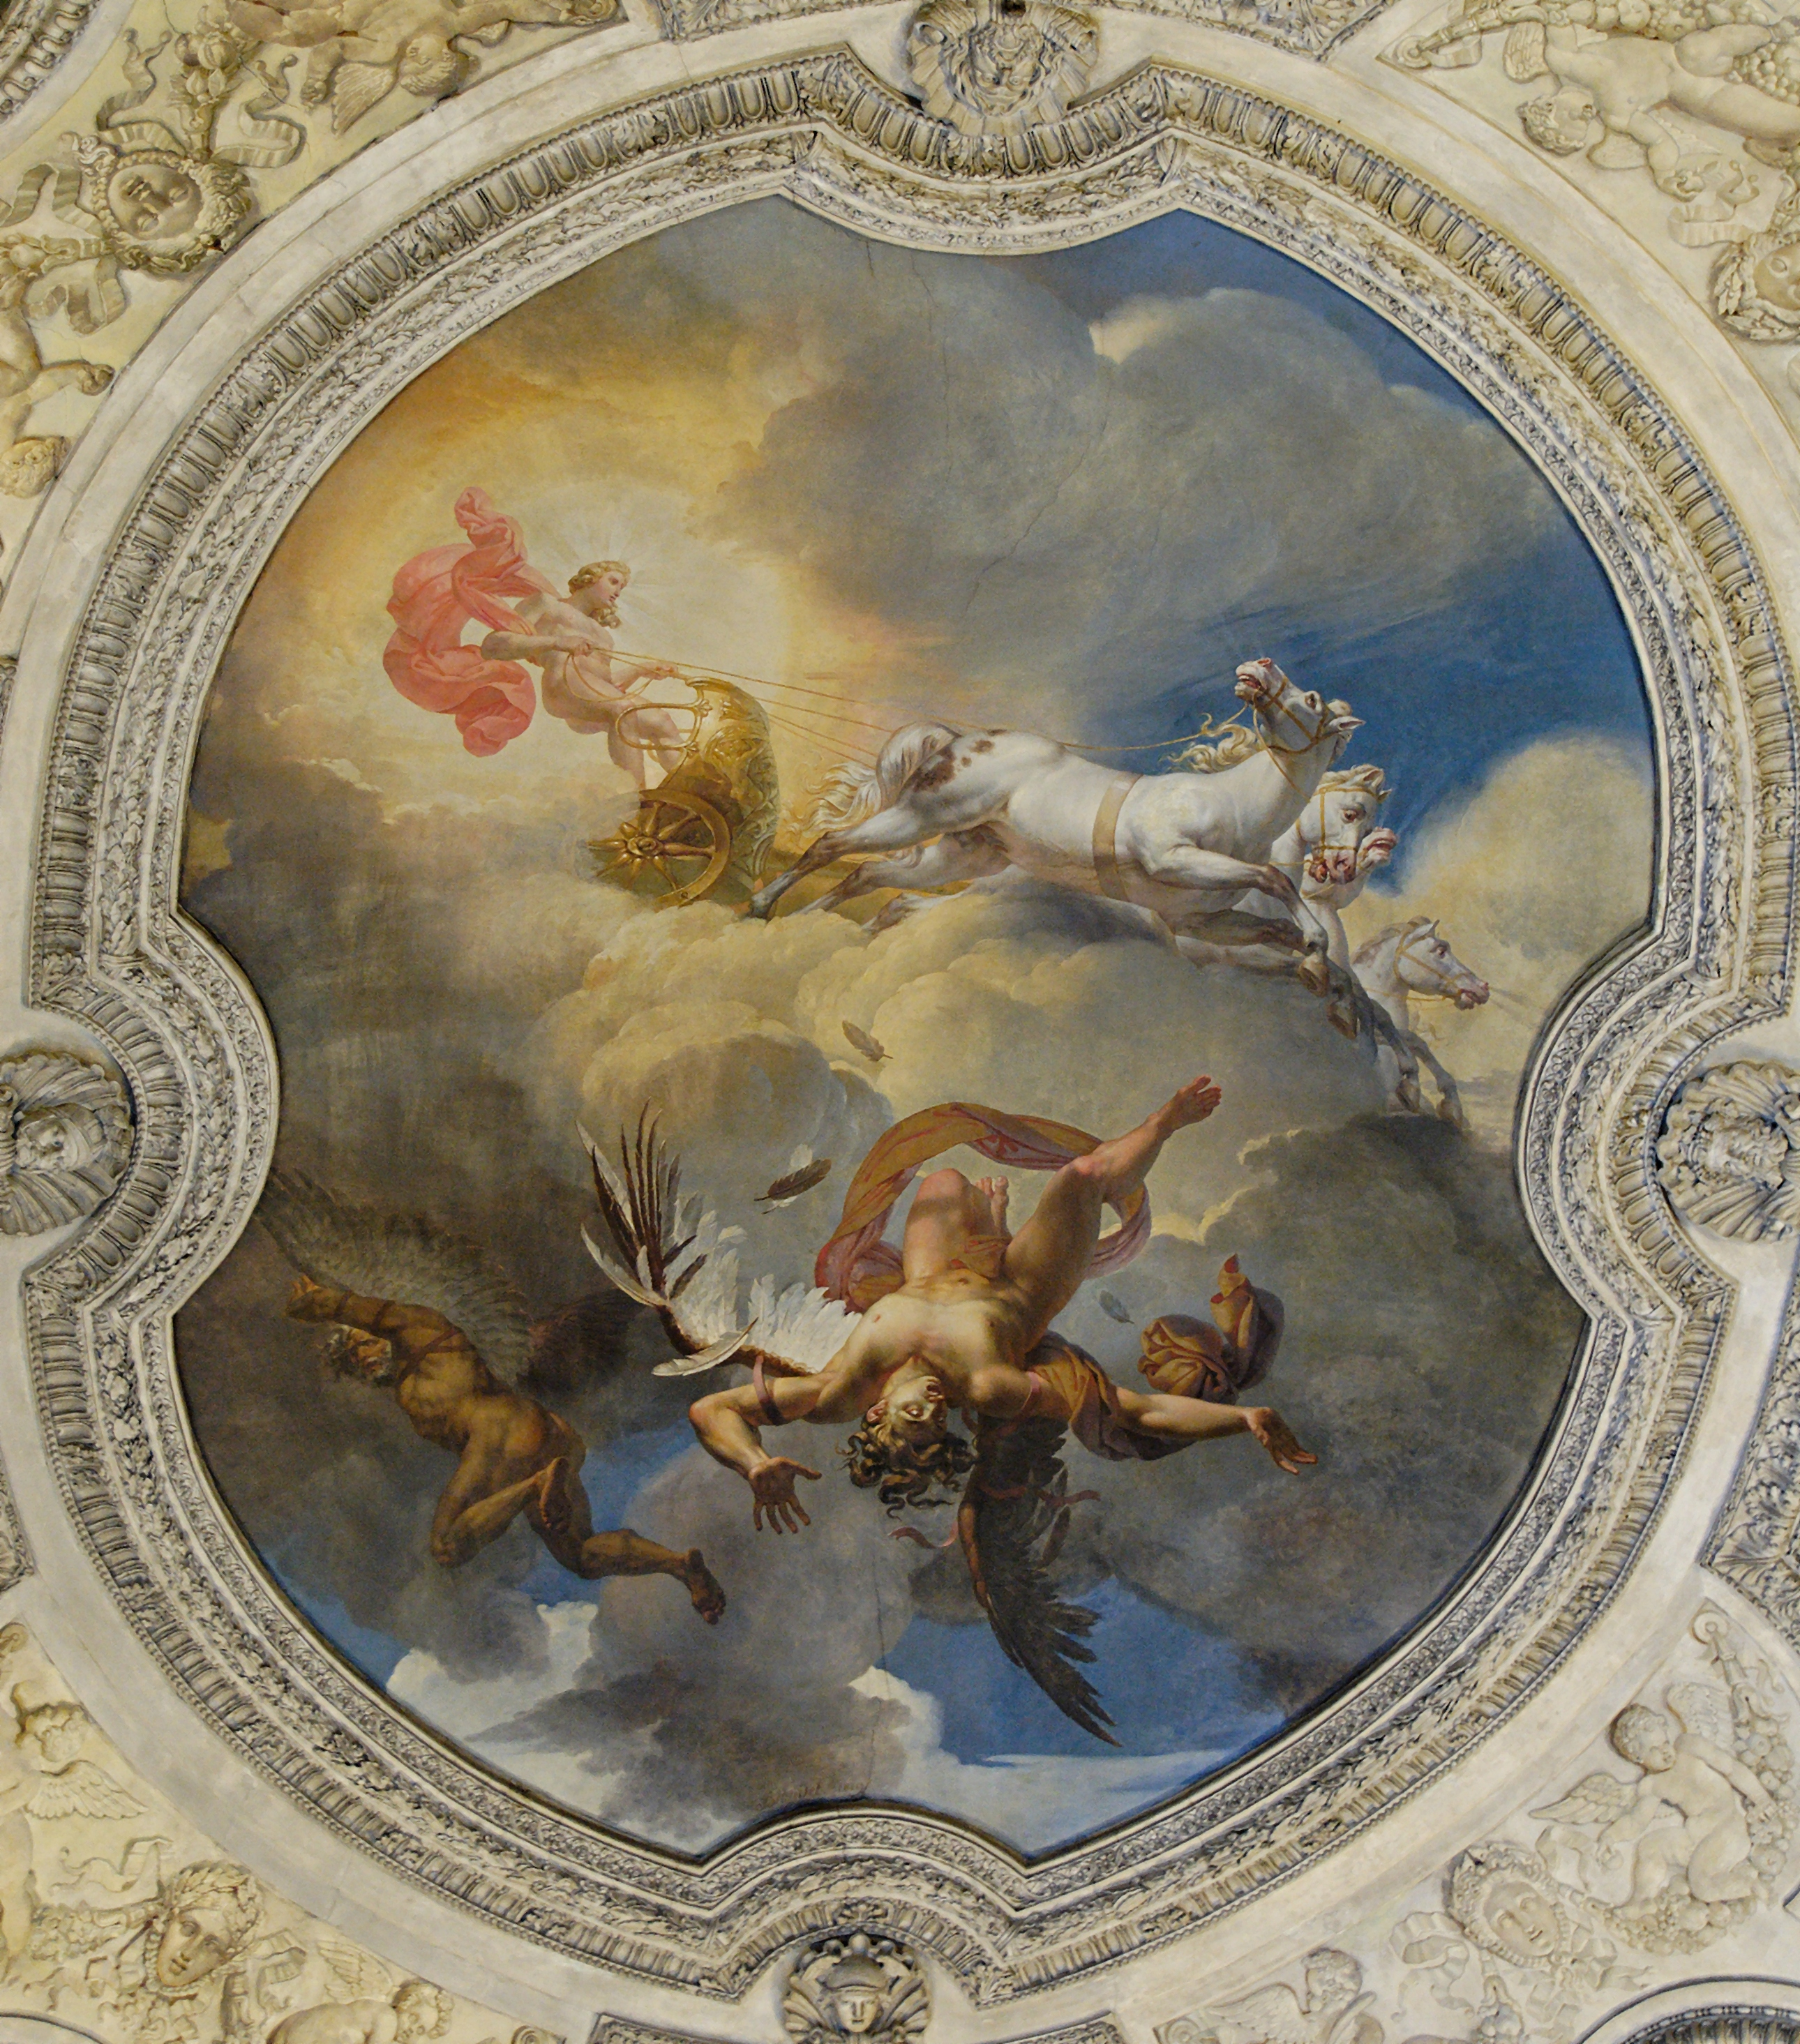
\includegraphics[width=0.5\textwidth]{fall-of-icarus.jpg}
	\EC
}

\frame{\frametitle{\bf 1450 CE: The dream of flight}
	
	\large
	
	\BC
	\BS Humanism and the Renaissance: flight as a dream... \\\BS
	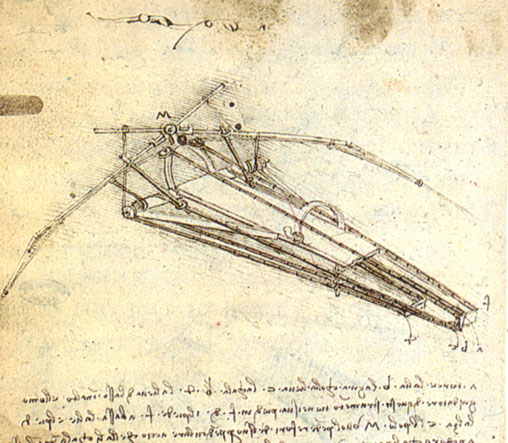
\includegraphics[width=0.5\textwidth]{da-vinci-flying-machine.jpg}
	\EC
}

\frame{\frametitle{\bf 1850-1900: The reality of flight}
	
	\large
	
	\BC
	\BS The Industrial Revolution: fly like the birds, dream of the Moon
	\BCC 
	\HC
	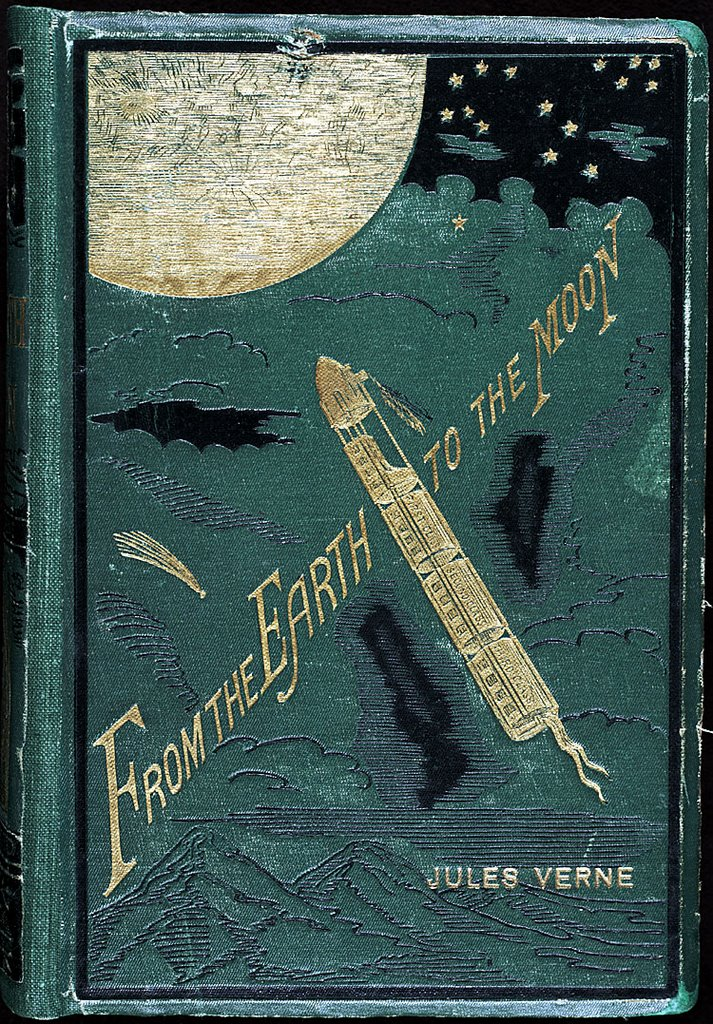
\includegraphics[width=0.8\textwidth]{earth-to-moon.jpg}
	\HC
	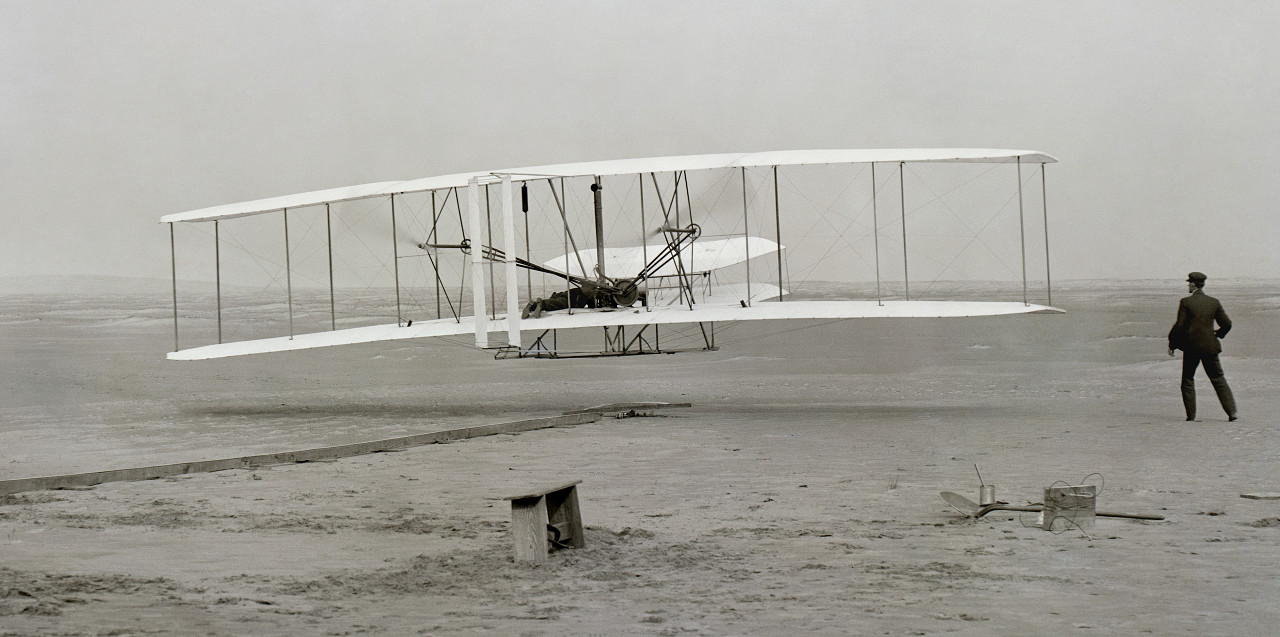
\includegraphics[width=1\textwidth]{wright-brothers-flight.jpg}
	\ECC
	\EC
}

\frame{\frametitle{\bf 1960's: to the Moon!}
	
	\large
	\BC
	\BS The space age: one small step for Armstrong... 
	\BCC
	\HC
	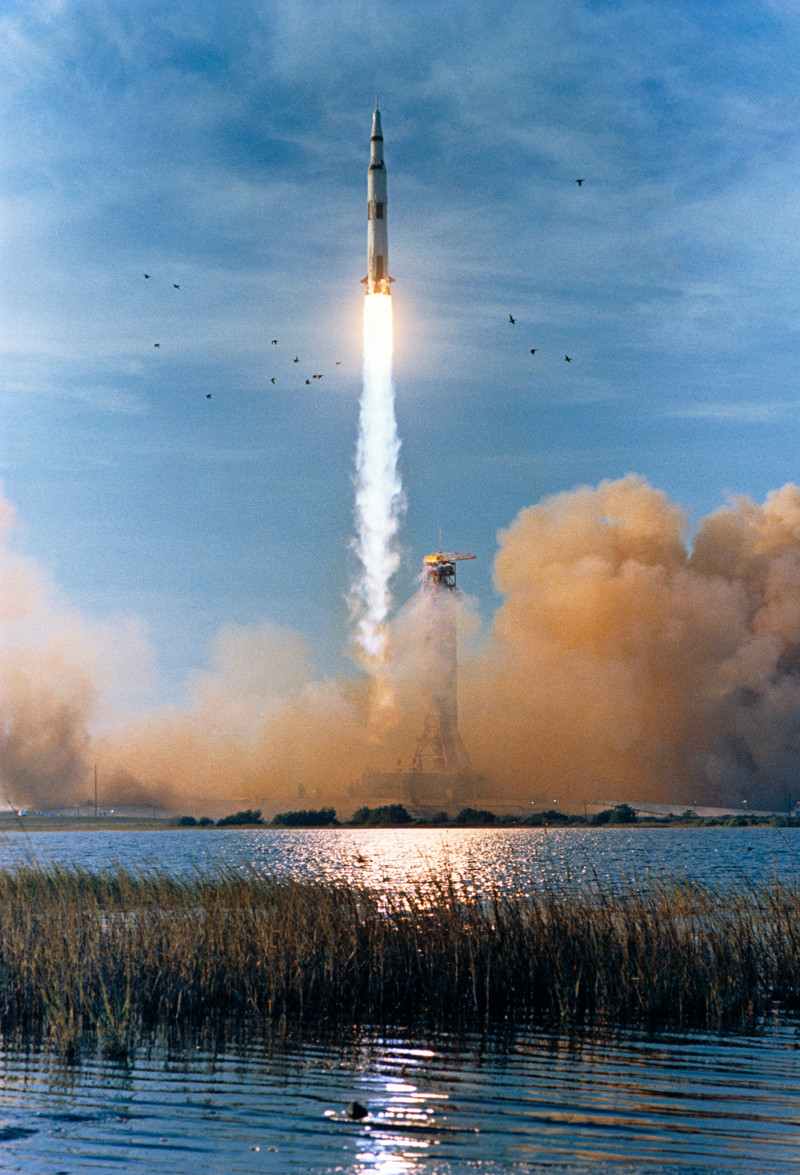
\includegraphics[width=0.8\textwidth]{apollo8-highres.jpg}
	\HC
	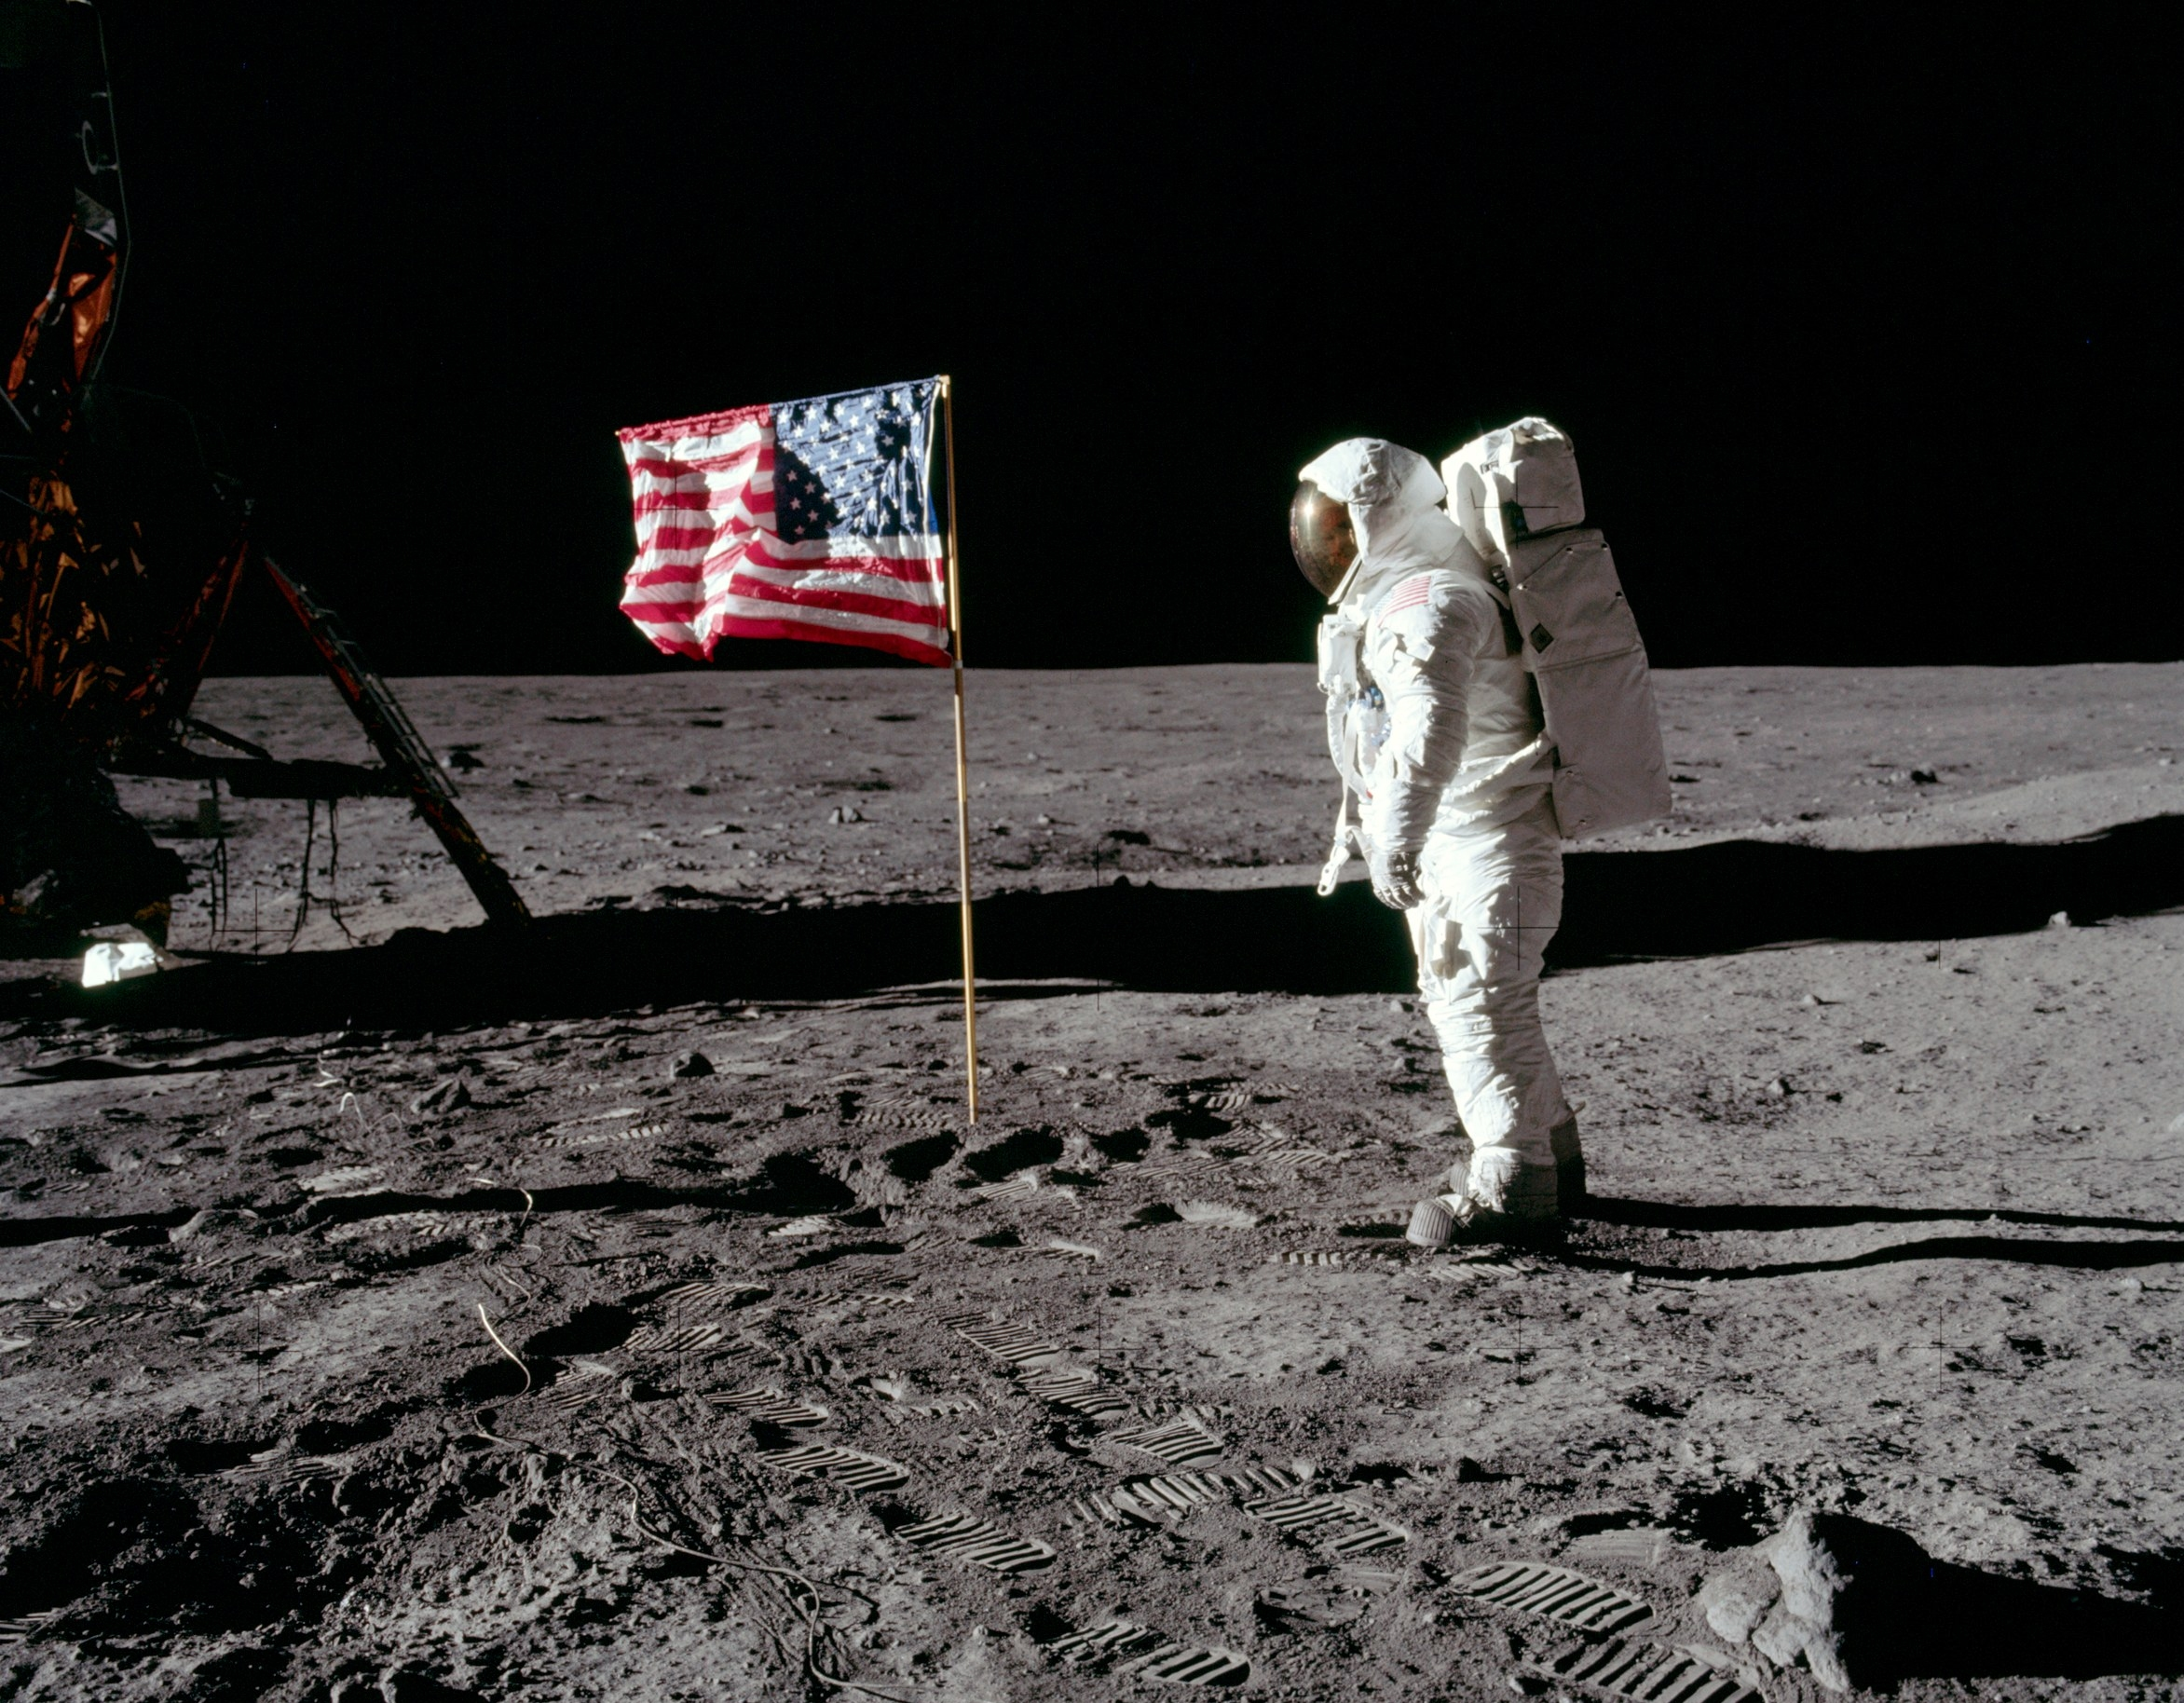
\includegraphics[width=1\textwidth]{apollo-11-landing.jpg}
	\ECC
	\EC
}

\frame{\frametitle{\bf Today: what next?}
	
	\large
	\BI
	\item What did we do on the Moon?
	\item What else have humans done in space?
	\pause
	\item Getting to the planets
	\item Getting {\color{Red}us} to the planets
	\item Getting to the stars
	\EI
	
	
	\BC\pause
	\Large \bf \color{D}The most important topic today, though, is your questions.
	
	
	\normalsize \color{E} Spaceflight is inspiring; what would you like to talk about?
	\EC
	
}

\frame{\frametitle{\bf Apollo 11: the Moon, at last!}
	On 20 July, 1969, humanity walked on another world for the first time.
	\BI
	\item Neil Armstrong and Buzz Aldrin descended to the lunar surface
	\item Michael Collins stayed in lunar orbit in the Command Module
	\item They stayed on the Moon for nearly a day, walking on the surface for two and a half hours
	\item They brought back around fifty pounds of moon-rocks
	\item Gallery of images: \url{http://www.hq.nasa.gov/alsj/a11/a11\_eva\_thumbs.html}
	\EI
}

\frame{\frametitle{\bf The remainder of Apollo}
	\BBC
	\HC
	\BI
	\item The USA launched seven more {\it Apollo} missions to the Moon.
	\item Six of them made it; one, {\it Apollo 13}, suffered from an explosion en route.
	\BI
	\item Its story was made into a wonderful film of the same name
	\EI
	\item 800+ pounds of moon rocks returned to Earth
	\item Dozens of hours spent on the lunar surface
	\EI
	\HC
	\BC
	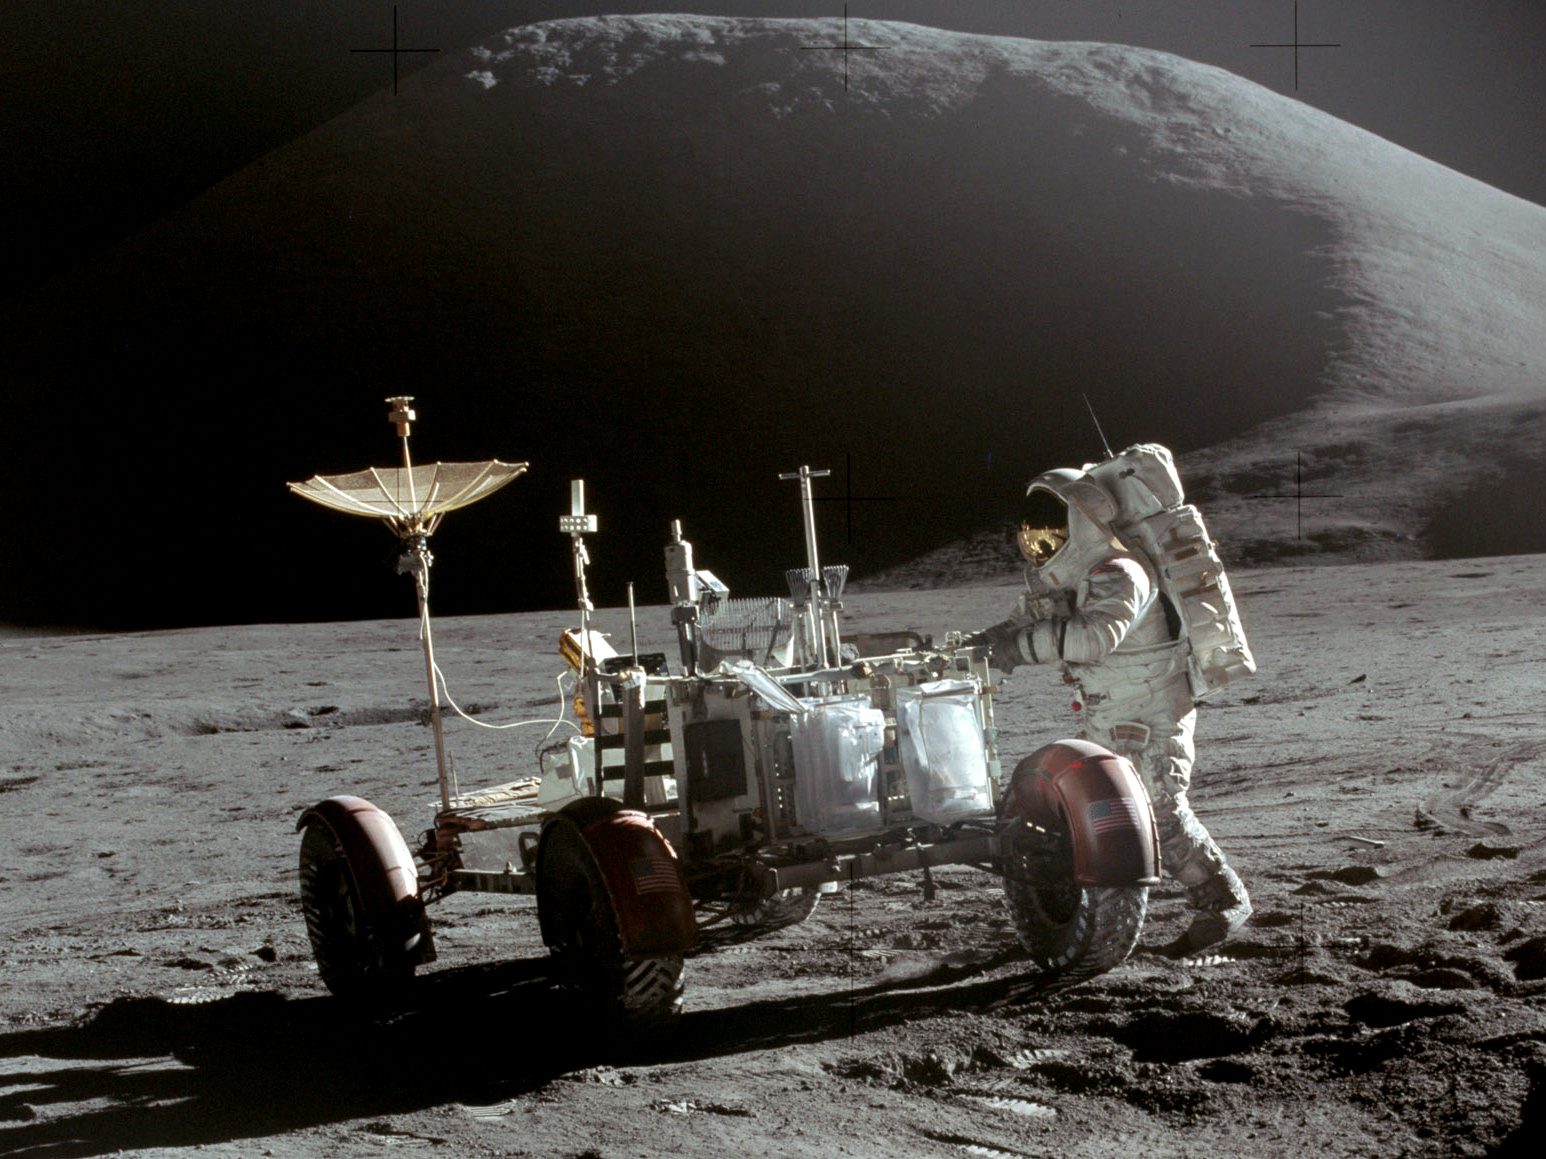
\includegraphics[width=0.9\textwidth]{lunar-rover.jpg}
	\EC
	\EEC
}

\frame{\frametitle{\bf Apollo 13}
	\BCC
	\column{0.3\textwidth}
	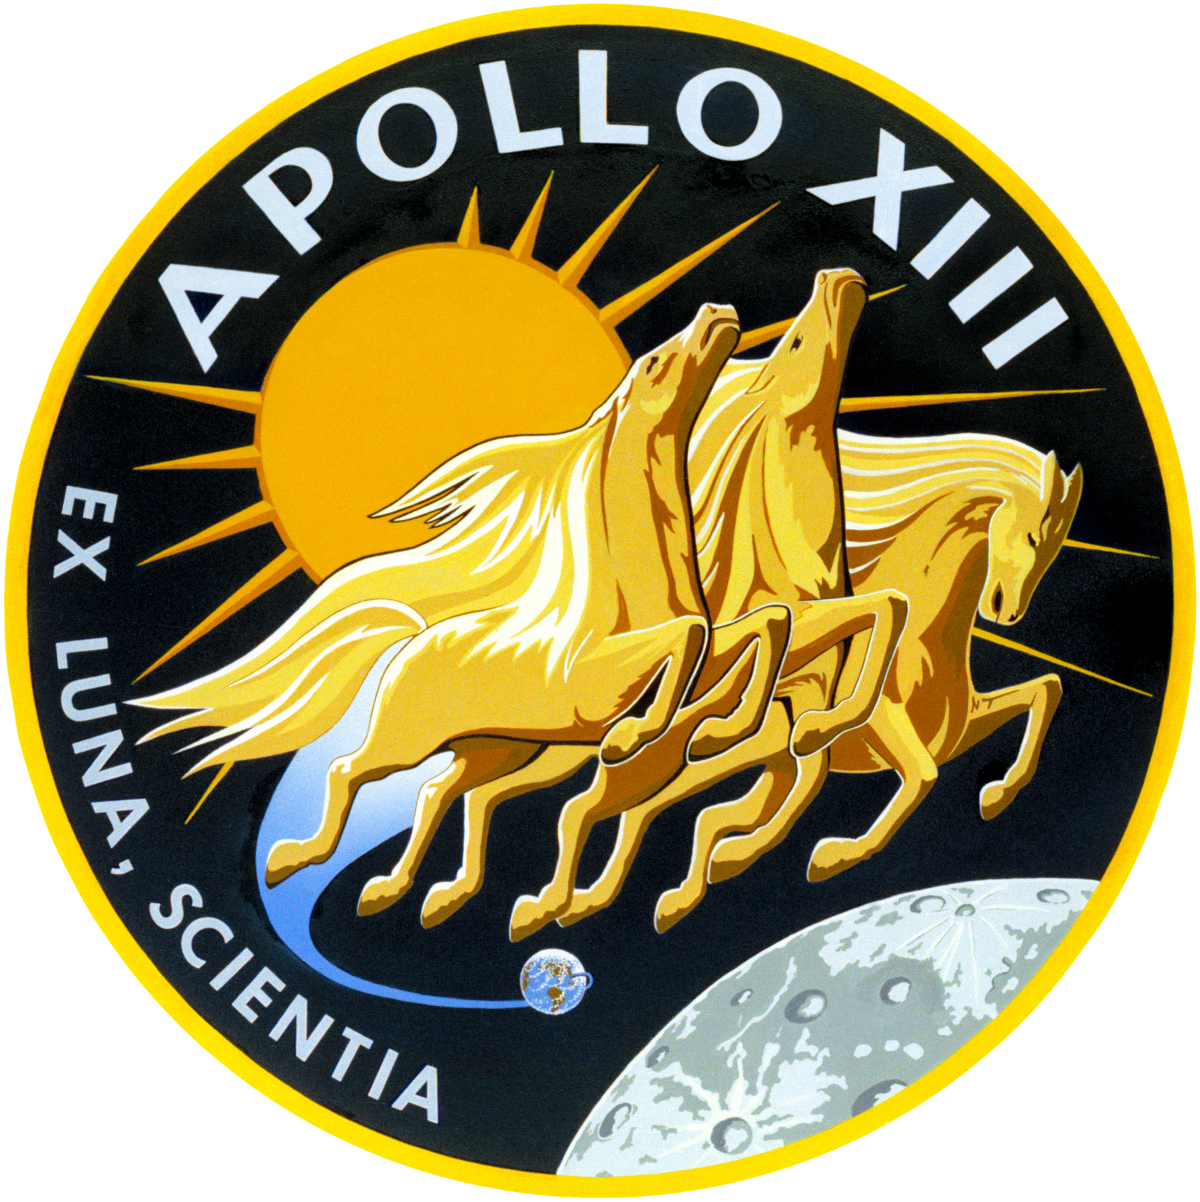
\includegraphics[width=1\textwidth]{apollo-13.png}
	\column{0.7\textwidth}
	\BI
	\item Oxygen is nasty stuff... \url{https://youtu.be/C3J1AO9z0tA?t=10}
	\pause
	\BI
	\item If you've not watched the film, you really should.
	\EI
	\pause
	\item The explosion happened while moving away from Earth
	\item They had to survive long enough to use the Moon's gravity to turn around
	\item Only cleverness and improvisation got the astronauts home
	\item \url{https://www.youtube.com/watch?v=1cYzkyXp0jg}
	\pause
	\item Humans aren't a successful species because we're good at what we're prepared for
	\item ... human intelligence lets us survive things we're {\it not} prepared for
	\EI
	\ECC
}


\frame{\BC
	\includegraphics[width=0.7\textwidth]{apollo-17.jpg}\EC
}

\frame{\BC
	\BBC
	\HC
	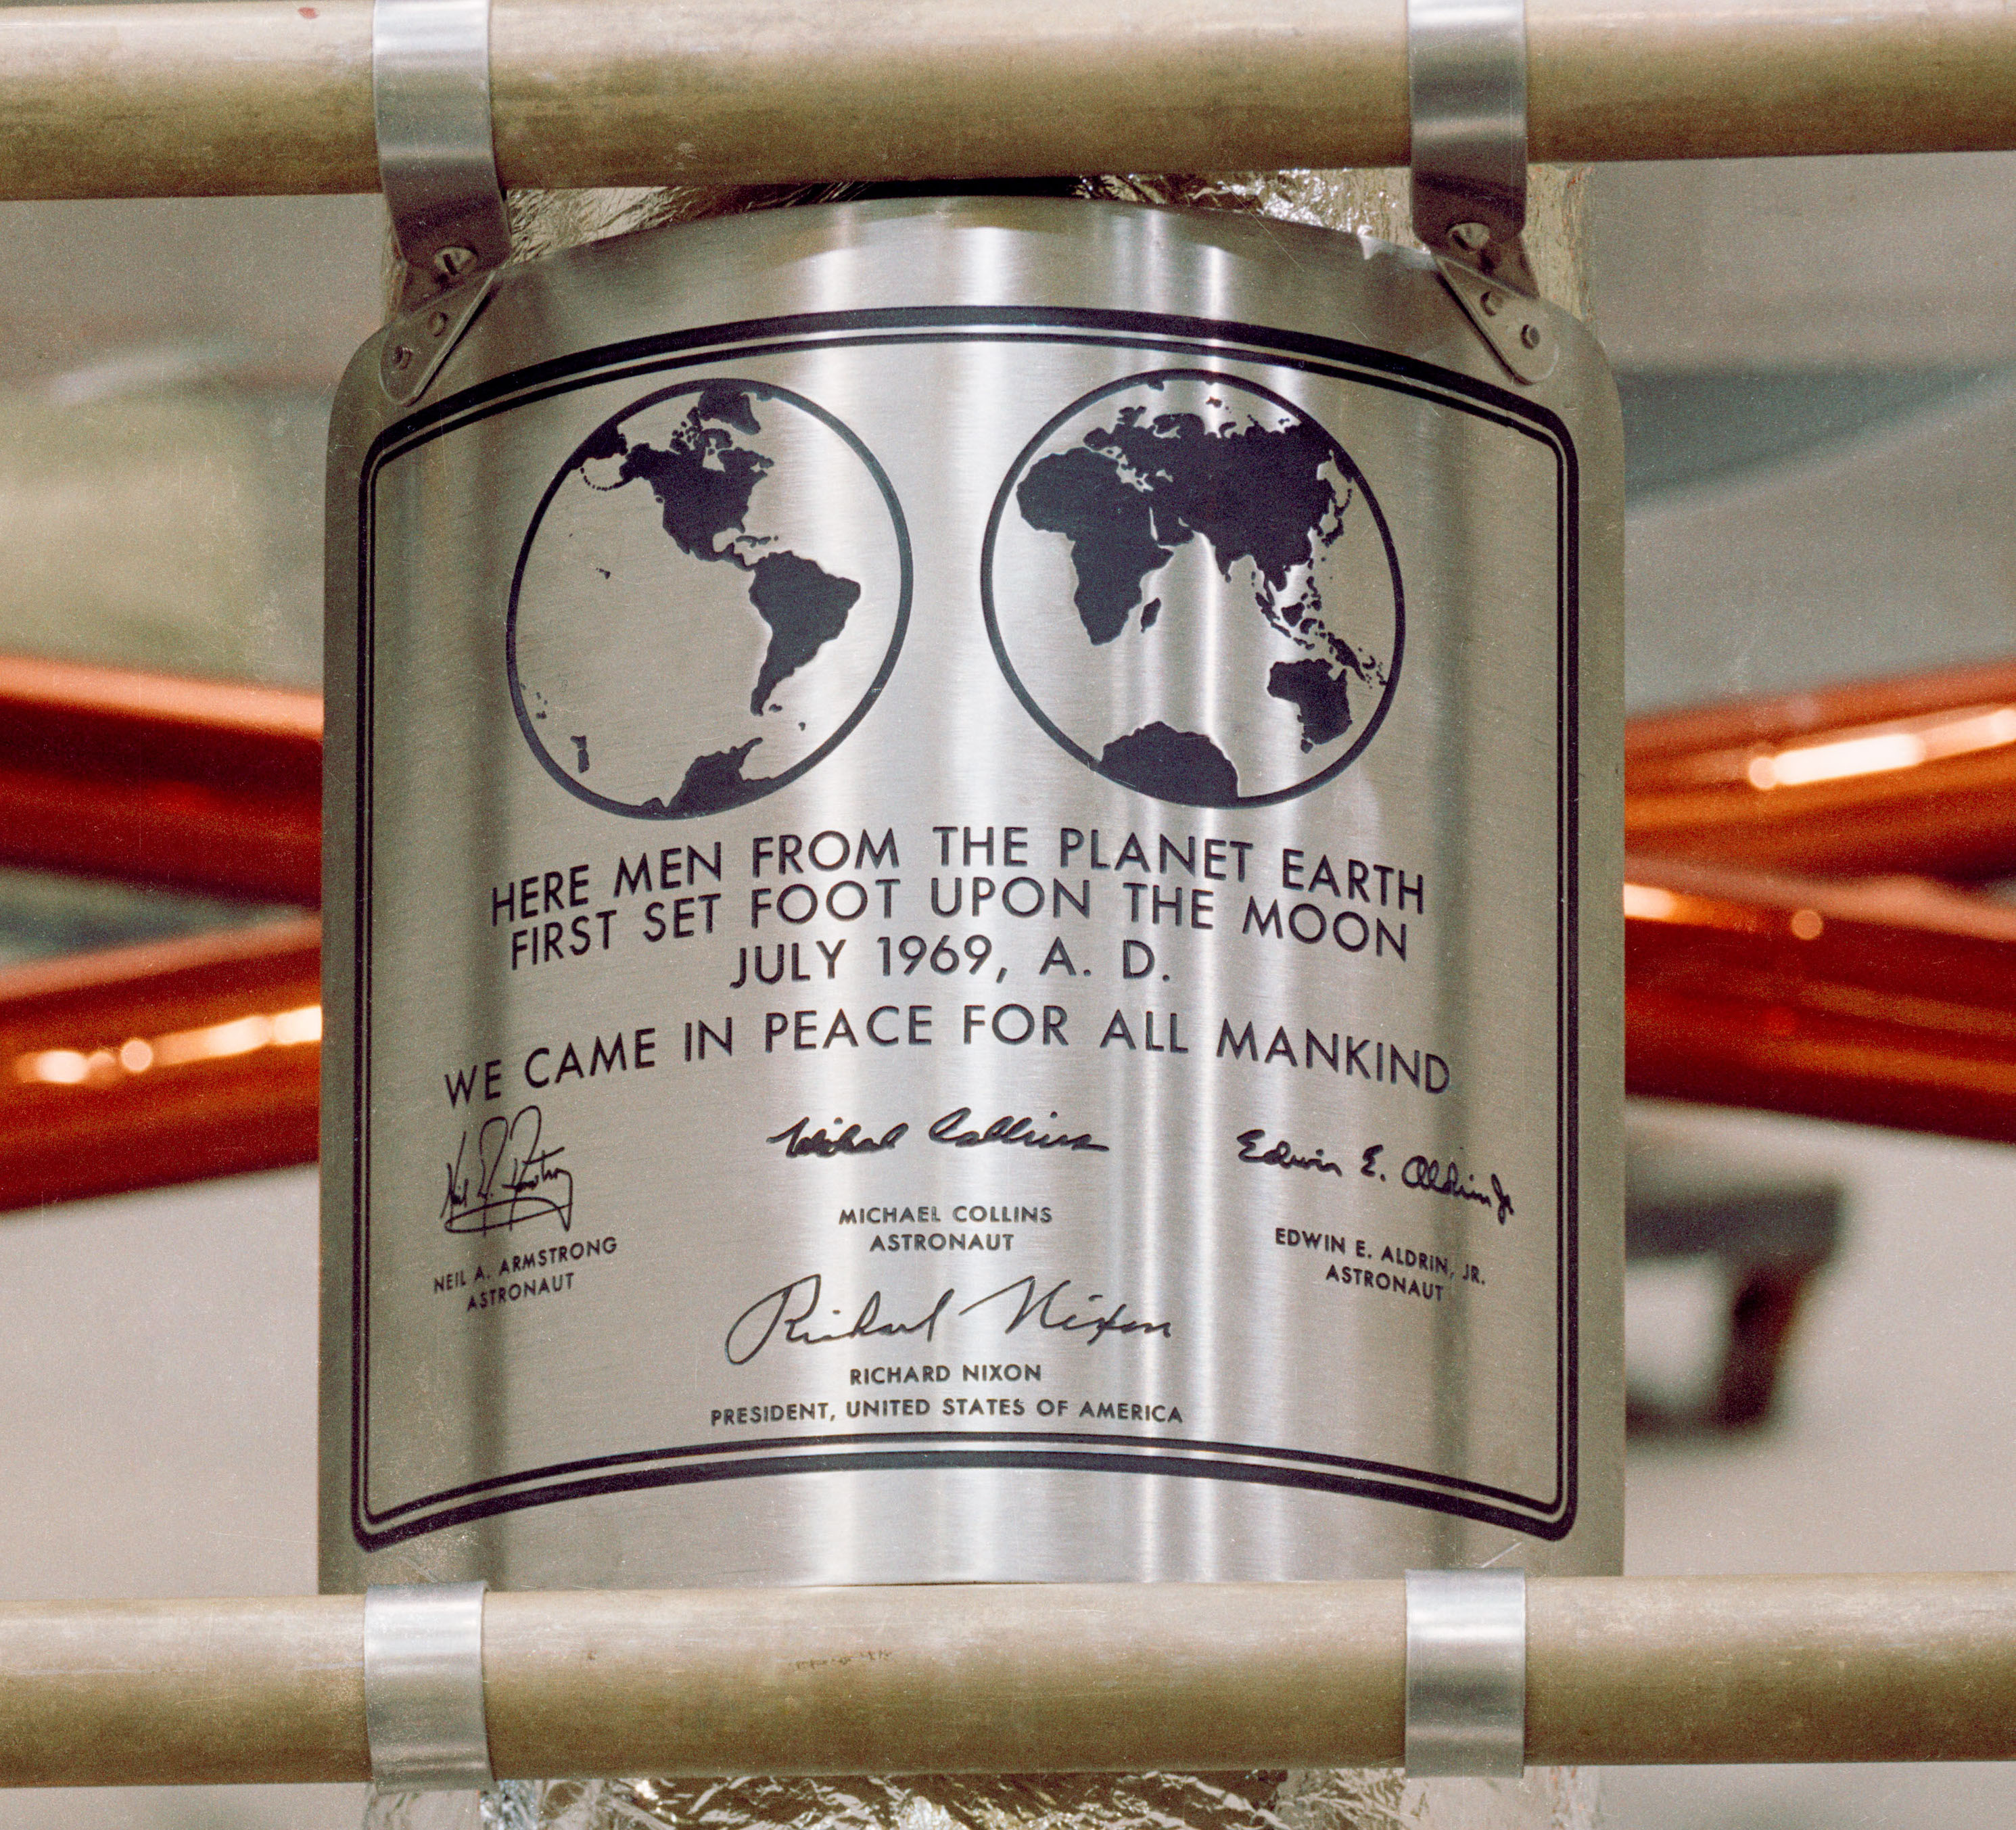
\includegraphics[width=\textwidth]{apollo-11-plaque.jpg}
	\HC
	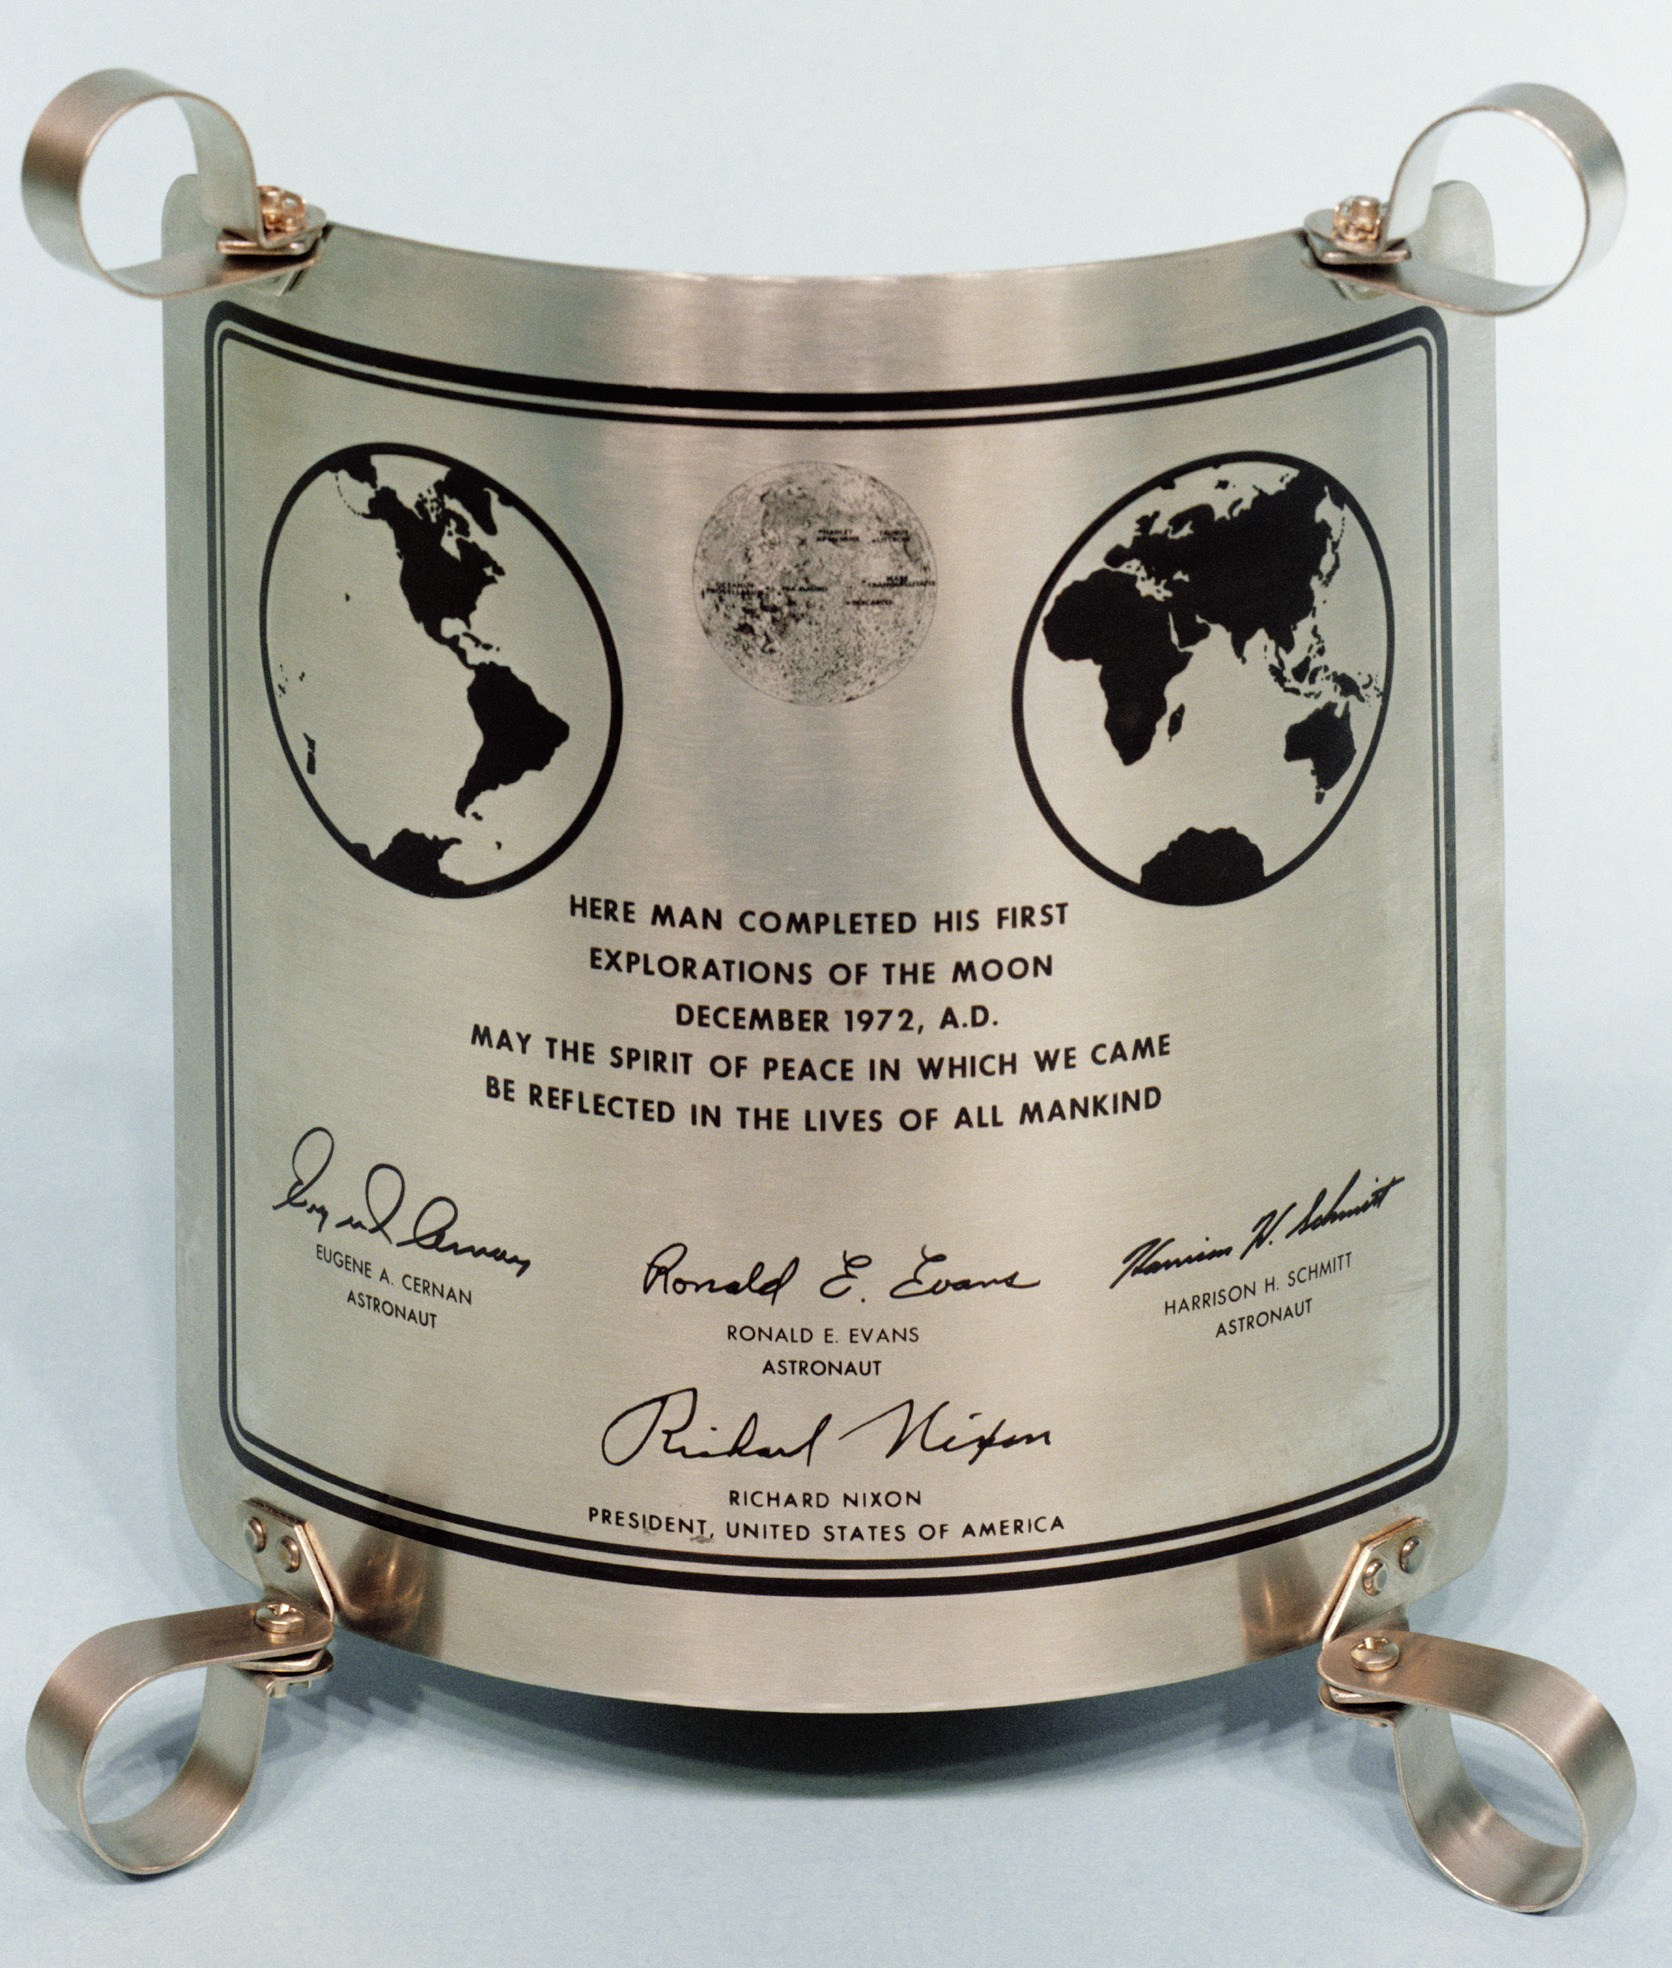
\includegraphics[width=0.9\textwidth]{apollo-17-plaque.jpg}
	\EEC
	\EC
}

\frame{\frametitle{\bf Not just the Moon}
	Kennedy called for the USA to go to the Moon in 1961. The last Apollo mission to the Moon was in 1972.
	
	\BS
	
	Meanwhile...
	\BI
	
	\item 1961: Soviets launch first Venera mission to Venus (it broke before arriving)
	\item 1962: TV satellite (USA); spy satellite (USSR)
	\item 1962: Americans launch Mariner 2, which flies by Venus (Mariner 1 failed)
	\item 1965: France launches a satellite
	\item 1965: Mariner 5 makes close pass by Mars \pause
	\item late 1960's: US sends Pioneer craft in solar orbit (some survived for 30+ years)
	\item 1970: Japan and China launch satellites\pause
	\item 2019: 9000 satellites launched, 5000 still up there, 2000 still working\pause
	\item ... we've gotten so good at this that ``space pollution'' is now an issue!\pause
	\item {\color{B} Satellite constellations (like Starlink) new source of light pollution}
	\item {\color{A} ``Anti-satellite'' weapons could set off a chain reaction making orbit very dangerous}
	
	\EI
}

\frame{\frametitle{\bf Robotic missions and the planets}
	\BI
	\item 1971: Mariner 9 enters Martian orbit
	\item 1972: US launches Pioneer 10-11, which exited the Solar System
	\item 1973: USA launches Skylab, which didn't hit anyone on the way down (sorry, kangaroos)
	\item 1974: Mariner 10 waves to Mercury
	\pause
	\item {\color{Red}1975: Docking between Soyuz-19 and Apollo 18}
	\pause
	\EI
	\begin{center}
		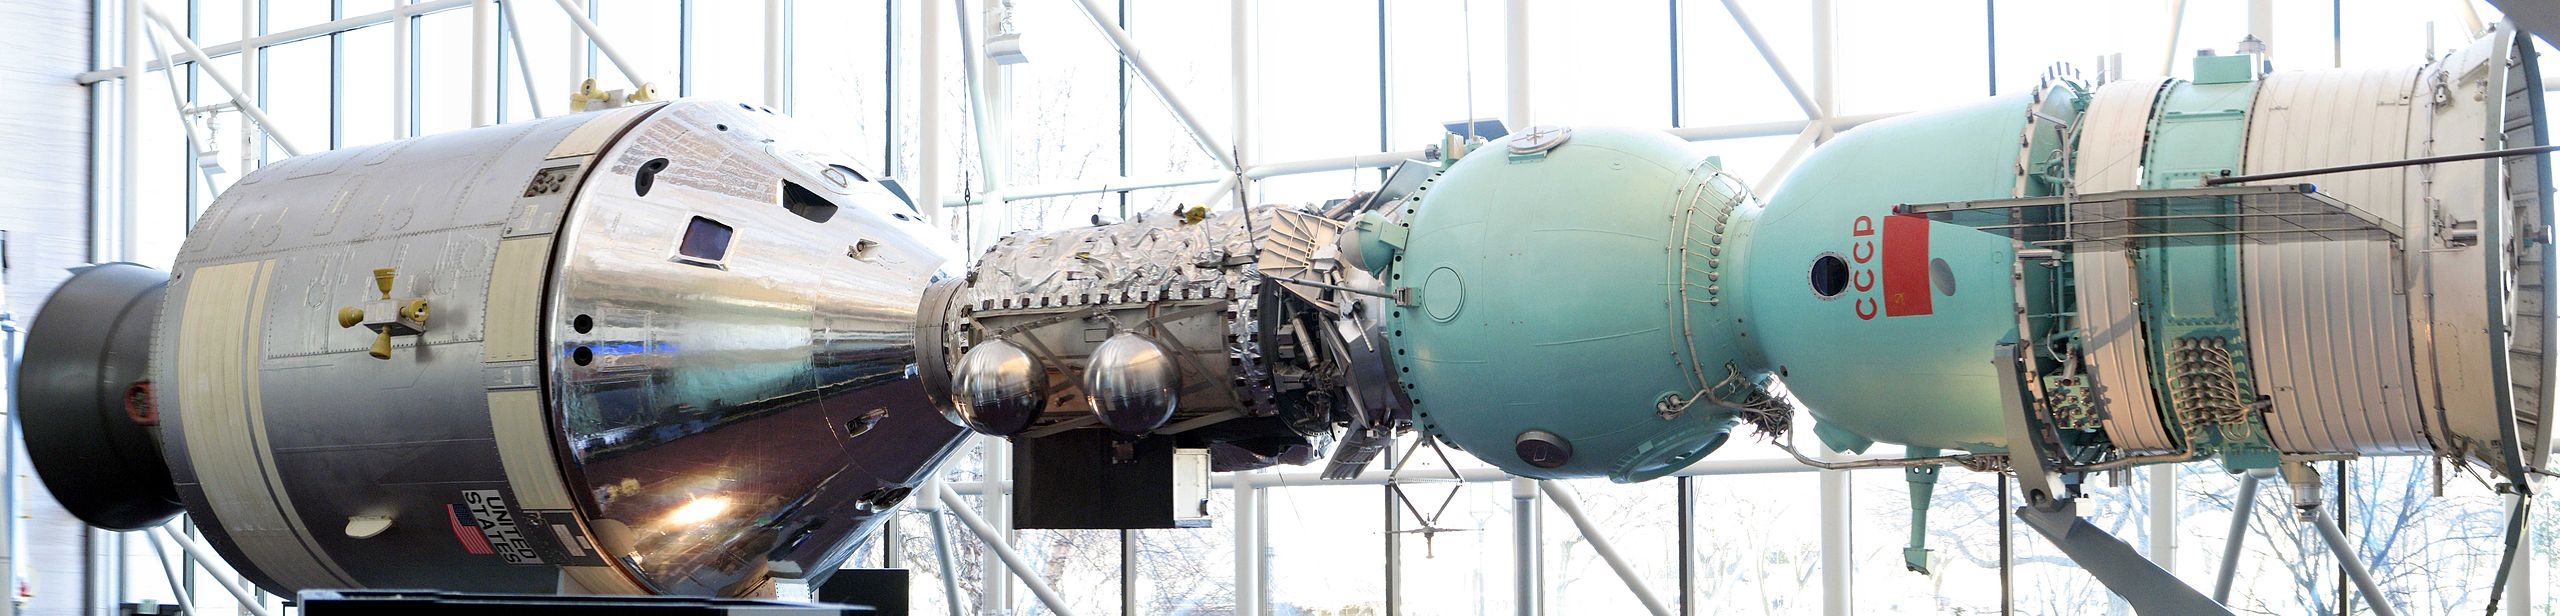
\includegraphics[width=\textwidth]{apollo-soyuz.jpg}
	\end{center}
}

\frame{\frametitle{\bf Robotic missions and the planets}
	\BI
	\item 1976: Viking 1 (USA) lands on Mars
	\item 1977: Voyagers 1 and 2 launched, passing by outer planets and leaving the Solar System
	\item 1981: Space Shuttle program begins
	\item 1986: USSR launches Space Station Mir (``Peace'' or ``World''); it crashes in 2001
	\item ... and more
	\EI
}
%
%\frame{\frametitle{\bf Return to the Moon?}
%	\BCC
%	\HC
%	\small
%	The Soviets nearly made it to the Moon, but gave up their project after the Americans ``got there first''.
%	
%	\BS
%	
%	After the end of Apollo, the Americans never went back to the Moon.
%	
%	\BS\pause
%	
%	Growing up in a NASA town, this was a sore point!
%	
%	\BS\pause
%	
%	Neither the Americans nor the Russians have designs on the Moon. However,
%	another nation is interested...
%	
%	\pause
%	
%	\BS
%	The Chinese space program has developed rapidly in recent years.
%	
%	\BS
%	
%	\BI
%	\item Robotic lander to the Moon: 2013
%	\item People to the Moon for good: 2030?
%	\EI
%	
%	\HC
%	\BC
%	
\includegraphics[width=0.7\textwidth]{clep-logo.jpg}
%	\EC
%	\ECC
%}

\frame{\frametitle{\bf Voyager 1: a history}
	\BI 
	\item 1977 (27): Launch (470 W power) \pause
	\item 1979 (29): Jupiter observations \pause
	\item 1980 (30): Saturn observations \pause
	\item 1990 (40): ``Pale Blue Dot'' portrait of Earth  \pause
	\item 1998 (48): Passes {\it Pioneer 10} at 69 AU; furthest Earth object \pause
	\item 2004 (54): 94 AU; enters termination shock (edge of ``heliosheath'') 
	\item 2012 (62): 121 AU; exits solar-wind bubble (``heliopause'')\pause
	\item 2017 (67): 141 AU; (19 light-hours) backup thrusters used for first time in 37 years; power down to 250 W \pause
	\item \color{B}2022 (72): 158 AU; 22 light-hours away\pause
	\item \color{C}2025 (75): 166 AU; Not enough power to run scientific instruments; science mission ends\pause
	\item \color{A}Around 2035 (85): Power insufficient to communicate with Earth \pause
	\EI
}


\frame{\frametitle{\bf The Space Shuttle}
	\large
	\BI
	\item Designed as a ``truck'' to low-earth orbit
	\item Great for human development (and spy satellites); not exciting for spaceflight
	\item Many, many flights -- most but not all successful
	\item \url{https://www.youtube.com/watch?v=AfnvFnzs91s}
	\pause
	\item \url{https://youtu.be/MWZs8l2AMps?t=8}
	\item Management science: big enterprises are {\it hard} when you must catch all mistakes
	\pause
	\item How can we go beyond LEO?
	\EI
}

\frame{\frametitle{\bf Why the Space Shuttle is not exciting}
	\BC
	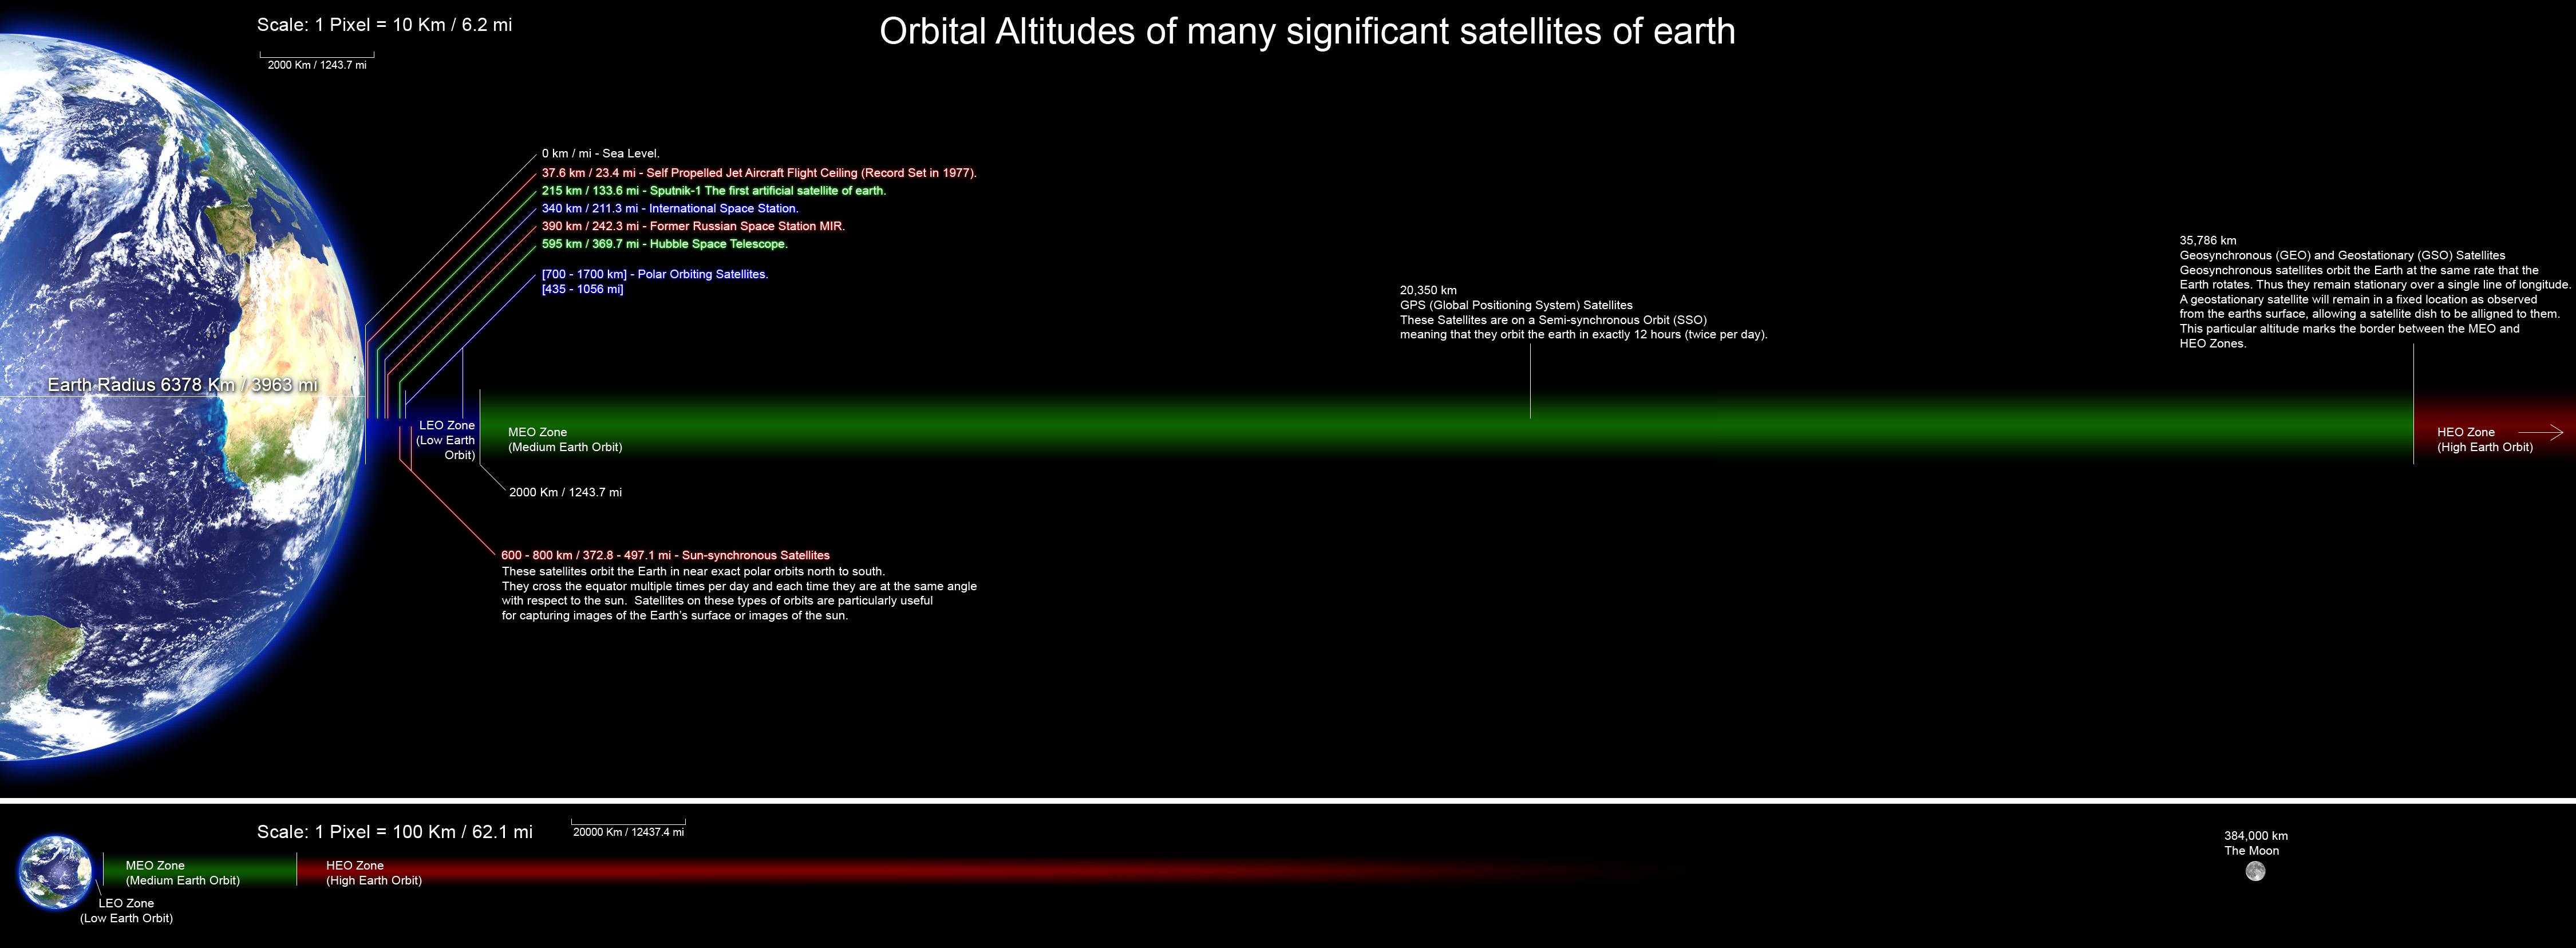
\includegraphics[width=0.95\textwidth]{low-earth-orbit.jpg}
	
	\BS
	\normalsize
	\url{https://upload.wikimedia.org/wikipedia/commons/8/82/Orbitalaltitudes.jpg}
	\BS
	\large
	
	\EC
}

\frame{\frametitle{\bf Going beyond}
	\large
	\BI
	\item Good news: the hard part is just getting off of Earth; after that it's much easier
	\item \url{http://i.imgur.com/AAGJvD1.png}
	\item Can use planets' atmospheres as a brake to slow down once we get there (no need for another huge rocket burn)
	\item What about getting people to Mars?
	\EI
}

\frame{\frametitle{\bf Humans to Mars?}
	\large
	\BI
	\item We've got one-ton robots on Mars; why are humans so much harder?
	\pause
	\item They're squishy
	\item They don't like radiation
	\item They want to come back (how much more $\Delta v$ is that?)
	\pause
	\item Possible solution: ``Mars Direct''-type plans
	\BI
	\item Send a robotic mission ahead of time
	\item The robotic mission prepares living space and sets up a nuclear reactor
	\item The energy from that reactor makes rocket fuel for the return trip out of Mars' atmosphere
	\EI
	\EI
}

\frame{\frametitle{\bf The bigger obstacle: cost}
	\large
	\BI
	\item Cost of Apollo program: \$200B
	\item Cost of one Shuttle launch: \$450M (or \$1.4B)
	\item Cost of {\it Curiosity} rover mission: \$2.5B
	\item Cost of crewed Mars mission: \$500B - \$1000B (?)
%	\item {\color{Red}Cost of {\it Mars Insight}: \$0.8B}
	\pause
	\color{A}
	\item Cost of US wars in Iraq: \$2500B-\$5000B
	\item Cost of Manhattan Project: \$25B
	\item US military budget per year: \$800B
	\pause
	\item Revenue lost from 2017 tax changes: \$1000-1500B (Senate Joint Committee on Taxation / Office of Management and Budget)
	\pause
	\color{C}
	\item US spending on healthcare (public and private) per year: \$4000B
	\item US spending on COVID response: \$4400B
	\item US gross domestic product per year: \$25,000B
	\item World GDP per year: \$96,000B
	\EI
	
	\BS\BC
	\color{D} There is a very real debate here about priorities!
	\EC
	
}


%\frame{\frametitle{\bf Mars InSight}
%	
%	\BC
%	\Large We landed another robot on Mars in 2018!
%	\BS
%	
%	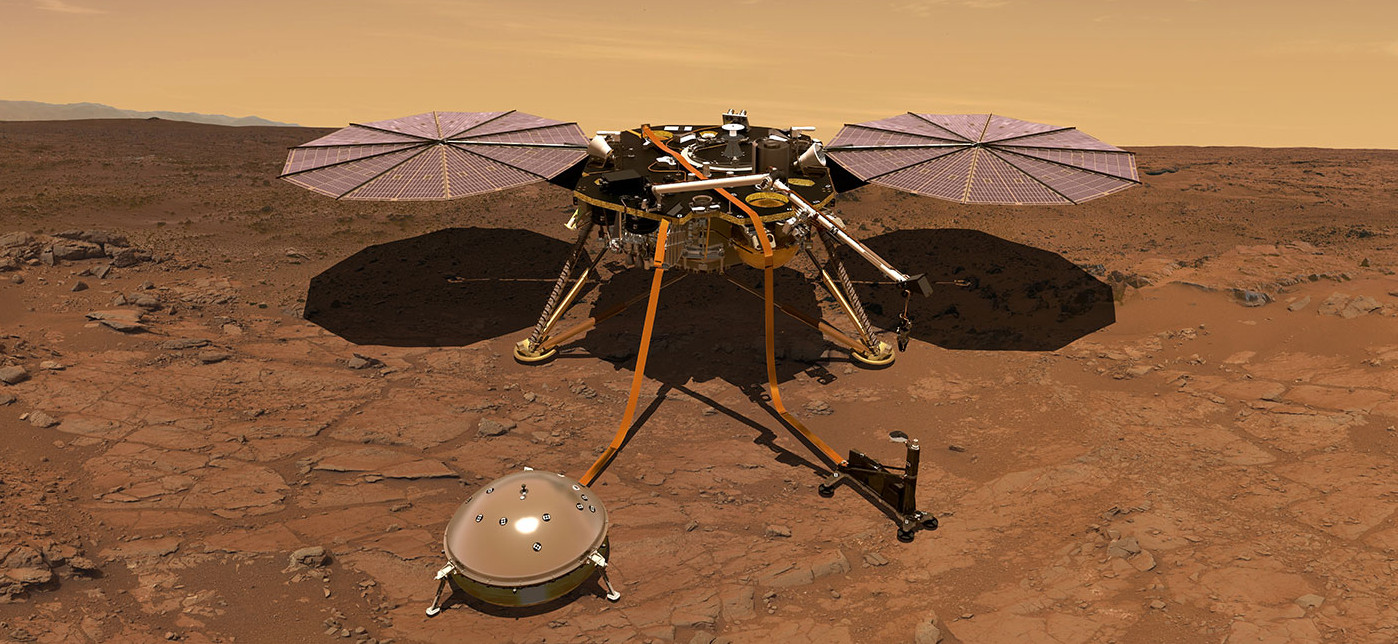
\includegraphics[height=0.4\textheight]{mars-insight.jpg}
%	\EC
%	
%	
%	\normalsize Mars InSight is a different sort of Mars robot.
%	Instead of driving around, it will stay in one place and probe details about planetary geology.
%	
%	\pause
%	
%	\BS
%	\BI
%	\item Seismometry: detecting marsquakes
%	\item Thermometry: how does heat flow through Mars?
%	\item Wobbleometry: how is Mars' mass arranged?
%	\item Retroreflectors -- surveying for the future!
%	\pause
%	\item Exploding meteor sonar -- mad science at work!
%	\EI
%}




\frame{
	\Large
	
	Is it important for humans to go to Mars?
	
	\bigskip
	
	\large
	
	\color{A}A: No; resources are limited and we have more important things to do on Earth\\\BS
	\color{B}B: No; we can explore just as well with robotic probes for a fraction of the cost\\\BS
	\color{C}C: Yes; science aside, sending humans to Mars advances the scope of human capability, in the same spirit as Kennedy's call for a moon mission\\\BS
	\color{D}D: Yes; there are things that only humans can do, and the extra cost is worth it in what we'll learn\\\BS
	\pause
	\color{E}E: Beam me up, Scotty; there's no intelligent life down here!
}



\frame{\frametitle{\bf Tsiolkovsky: we just need better fuel!}
	
	
	\BS

	\BS
	
	\normalsize
	% Please add the following required packages to your document preamble:
	\BC% \usepackage{booktabs}
	\begin{tabular}{@{}ll@{}}
		\toprule
		Fuel exhaust speed            & Fuel needed              \\ \midrule
		1000 km/hr                    & 300 million billion tons \\
		2000 km/hr                    & 5.5 million tons         \\
		3000 km/hr                    & 680,000 tons             \\
		5000 km/hr                    & 3100 tons                \\
		9000 km/hr (solid rockets)    & 87 tons                  \\
		15400 km/hr (hydrogen/oxygen) & 13 tons                  \\
		104000 km/hr (ion thrusters)  & 470 kilograms      \\
		\toprule
	\end{tabular}
	\EC
	
	If we could just do better than hydrogen/oxygen rockets, we'd be in business...
	
	\BS
	
}

\frame{\frametitle{\bf Solutions to go beyond...}
	
	\large
	\BI
	\item Higher exhaust-velocity rockets: nuclear propulsion?
	\item Dealing with human lifespans
	\pause
	\item Sudden vs. gradual advancement -- what's happened in a century?
	\pause
	\item More next time!
	\EI
	\pause
	\url{https://www.youtube.com/watch?v=S-WRKeSerUE}
}




\end{document}
